\documentclass[final]{scrartcl}

\usepackage{graphicx}

% Custom package with preamble definitions
\usepackage{mystyle}

% Custom commands for typesetting specific names
\usepackage{mycryptonames}

\renewcommand{\circ}{\rightarrow}

\usepackage{biblatex}
\addbibresource{references.bib}

%\titlehead{}
\title{Companion to Cryptographic Primitives, Protocols and Proofs}
\author{Chris Brzuska\thanks{chris.brzuska@aalto.fi} }
\author{Valtteri Lipiäinen\thanks{valtteri.lipiainen@aalto.fi} }
\affil{Aalto University, Finland}
\date{\today}

\begin{document}

\maketitle
\begin{abstract}
    This book gives an introduction to cryptography, starting from modelling security and ending with technical proofs of security. To reach this end point, the necessary definitions and notations are introduced. Security games are used to model security, and the oracles involved are defined in pseudocode. Various cryptographic primitives are defined precisely in a unified manner, and relationships between these primitives are proven rigorously.

    The focus of this book is on presenting foundations and definitions in a bottom-up manner, while being easy to use as a reference document. The foundations, definitions and techniques of this document give you the necessary technical background to understand common cryptographic primitives and be able to argue about them rigorously.
\end{abstract}
\clearpage

\tableofcontents
\clearpage

\section*{Preface}
This book was written with the following two guiding principles.
\begin{itemize}
\item[(1)] Definitions are easy to find fast
\item[(2)] All necessary \emph{technical} content is presented in a bottom-up fashion. 
\end{itemize}
The book thus represents the dependency of definitions, showing which definition builds on which other definition. We consider this a useful way to structure knowledge.

The sections of the book are relatively self-contained, to make the document easier to use as a reference. Each section starts with an explanation of what it contains, why you might want to read it, and how it relates to other parts of the document. We will also provide cross-linkings between the sections where relevant.

Section \ref{section:foundations} goes over foundations. Section \ref{ssec:security-foundations} provides background on how security is modelled. The later sections go over further details, including discussion of models of computation and runtime. Section \ref{section:definitions} contains notation and definitions necessary for security definitions. The security game framework for giving security definitions is covered in Section \ref{ssec:security-games}. Section \ref{section:primitives} gives security definitions for a range of cryptographic primitives. Section \ref{section:theorems} contains statements of results in cryptography, and Section~\ref{section:proofs} proves some of them. Between these two sections, Section \ref{section:proof-writing} gives some background on proof techniques.

If you find typos, have ideas for improvements, or think we have deviated too far from our guiding principles, you are very welcome to write to Chris Brzuska or Valtteri Lipi{\"a}inen. The people reading this document have varying backgrounds, so it would be helpful to include your background in the feedback. We attempt to provide links between parts of the book throughout. If you feel some useful pointer is missing, this would be very useful feedback to get.

\clearpage
\section{Foundations} \label{section:foundations}
In cryptography, we want to make statements such as the following:
\begin{quote}
No adversary running in time at most $t$ can break the system with probability greater than $\epsilon$.
\end{quote}

There are many layers to this statement. You might just argue informally that a system is secure, without being precise about what you are trying to prove. We believe this is a bad approach, and is prone to mistakes. This document introduces a more formal way of dealing with security, which requires careful consideration of what security statements like the one above mean. We start off by discussing how we model security. We explain what exactly we mean by an adversary, what a cryptographic system is and what it means to break it. These concepts are useful on their own, but for a more thorough understanding we have to discuss more foundational issues. We borrow from computer science and mathematics to explain what we mean by algorithms, how we measure their run-time, and how we reason about probability. In addition, we elaborate on two topics in cryptography: the need for assumptions in proofs of security, and describing larger systems by composing modular packages.

Reading this section will help you develop a formal understanding of the concepts this book deals with. However, it isn't necessary to read it, at least to start with. The parts from the definition section on are self-contained. If you like to learn by doing, it might be better to start doing the exercises, and return here if you get confused by something. You can also start off reading the parts that interest you the most. We provide forward and backward pointers throughout the document.

This section deals with mathematics and computer science, so we will add remarks for those with a background in these areas as we go. If you study another subject, both or neither of these comments might be useful to you.    
\subsection{Security}\label{ssec:security-foundations}
The concepts of a cryptographic system and an adversary are foundational to capturing security of cryptography. We already referred to adversaries and cryptographic systems in the statement at the very beginning of this section. So, now, let us start our discussion of security by elaborating on what we mean by the \emph{adversary} concept and by the concept of a \emph{cryptographic system}.

Cryptography studies the security of systems, functionalities and communication from adversarial interference. It is helpful to think of such situations as dividing agents into two groups: the system with its users, and the adversary. The system has some functionality that its users want to use. This functionality includes correctness (e.g., an encrypted messaging application shall transmit messages to the intended recipient), but it also includes some intuition of what it would mean to break the security of that functionality (e.g., unwanted access to the messages by third parties). It would be impossible to study the security of such a system without also considering the agent that tries to break the security. We call this agent the adversary.
\begin{quote}
    Cryptography studies the interplay between the system and the adversary.
\end{quote}


So far, our concepts have been rather general, since there are countless different types of security we might wish to study. The concepts are easier to understand with a concrete example, so let's quickly go over what the Transport Layer Security (TLS) protocol is, and what sort of security we want to define for it. The TLS protocol secures most of our internet communication. To simplify, the functionality of TLS is to send messages over the network \emph{securely}. But what does secure mean? In the case of TLS, there are three different security properties we want for this functionality. First, we want \emph{authentication}, meaning that we can be sure of the identity of the agent sending a message. Second, we want \emph{integrity}, meaning that the messages are not modified between being sent and being received. Thirdly, we want \emph{confidentiality}, meaning that the contents of the message can not be seen by anyone expect the intended recipient. These concepts are still quite vague. The aim of the course is to clarify what exactly these types of security guarantees mean, and how we can prove that they hold (and under which assumptions). But before we go into further details, let's discuss security definitions at a more general level.

\paragraph{Security Definitions} What is a good security definition? We can define any number of different security notions. Therefore, when putting forward a new security notion, we should explain why it is useful, why it captures what we aim for and how it differs from ones that have been defined before (if any). A good security definition (1) has a clear conceptual motivation, (2) has a clear description, (3) comes with a discussion of necessary, arbitrary and convenient choices as well as (4) a discussion of advantages/disadvantages compared to other definitions.

Security definitions are necessarily intertwined with a notion of an adversary. To clearly understand security notions, we also have to have a clear understanding of the adversary. The adversary is the agent that tries to break the security of a system. There are two things that go into breaking the security of a system: access to the system and what is done with that access. We model the \emph{adversary} as an algorithm that gets some inputs from the system and returns something. We call the inputs that the adversary gets the \emph{adversarial capabilities}.
It depends on the situation being studied which capabilities the adversary has, and the capabilities have to be specified when defining a security notion. It is very common for the adversary to have the capability to read any messages sent over the network or even to entirely control the network traffic. There are also more specialized capabilities that an adversary might have, including being able to choose which messages a client sends (partial knowledge and/or control over the message content as, e.g., in the case of cookie-forwarding) or getting to see the outputs of a function for chosen inputs.

\begin{quote}
    How should we choose the adversarial capabilities?
\end{quote}

An important insight (on which we elaborate below) is that we do not know what the exact capabilities of a real-life adversary are.
Cryptography has to protect against attacks that even the designer of the system has not thought of.
Therefore, in our specifications of adversarial capabilities, we will typically \emph{over-approximate} a bit.
For example, we say that a network adversary can drop, re-order, delay, re-route and replace all network messages.
In a real-life attack scenario, an adversary can typically only perform such actions partially.
For example, the adversary might have only access to part of the network and might only be able to inject message but not be able to block all other messages.
Unfortunately, capturing the \emph{exact} attack capabilities of various network adversaries might
be impossible.
So, if we manage to specify a \emph{bigger} set of adversarial capabilities that comprises all network attacks that might be carried out, then we can consider such a set of adversarial capabilities as \emph{sufficiently strong}.
If we can show security against such a strong adversary, then, in particular, the protocols we build are secure also against weaker (realistic) adversaries which only have a subset of the capabilites. To summarize,
\begin{quote}
    in a good model, the adversary's capabilities can be \emph{more} than in real-life, but \emph{should not be less}.
\end{quote}
This sentence is an excellent summary for decision-making for whether or not to include a certain capability into the model. I.e., it is always good to be on the side of allowing the adversary \emph{more} rather than less. However, this principle is a bit too simple on its own and needs to be complemented by a second principle. Consider, for example, the situation where a user is coerced into revealing its key to the adversary. In this case, the adversary can impersonate the user, send messages on their behalf and read all their communication. However, we might have a feeling that this is not actually an attack against the \emph{cryptographic system} itself, but rather an attack onto the circumstances in which the system is used. In any case, our cryptographic system cannot provide security in this situation and thus, we have to exclude this attack from the model. We call attacks against which \emph{no} cryptographic system can protect \emph{trivial attacks}, and the second principle for adversarial capabilites states that
\begin{quote}
    in a good model, there are no trivial attacks.
\end{quote}

Similarly to being unable to estimate precisely the adversarial capabilities, we also do not know in advance what the adversary will do.
That's why we model the adversary as a general algorithm, without specifying what that algorithm does, and we would like to state that we provide security against any adversary as long as the adversary only uses the allowed adversarial capabilities (inputs from the system).
However, cryptography can typically be broken if an adversary invests \emph{an infeasible amount of time}, for example by trying out all possible keys.

\begin{quote}
    Our models provide security against arbitrary \emph{efficient} adversaries.
\end{quote}
Moreover, cryptography can typically be broken with some very small probability, e.g., if the adversary guesses the key correctly.
So, when we say that \emph{a system is secure}, then this typically means that

\begin{quote}
    \emph{all efficient
        adversaries} only have \emph{very small probability} in breaking the system.
\end{quote}
The terms \emph{efficient} and \emph{small} can be interpreted in different ways.
The interpretation this course uses is discussed in Section \ref{section:definitions}.

\paragraph{Proofs}
In addition to defining notions of security, we want to prove things about the security of specific systems.
Showing that an attack works against a system is typically easy: one executes the attack and thereby
convinces the observer that the attack succeeds.
When we design secure systems, we want to do the opposite: we want to show that no attacks against the system exist.
This is tremendously difficult, since there is an \emph{infinity} of attack strategies.
How can we show that none of them work?
Even if we are precise about the adversary's attack capabilities, there are still an infinity of
strategies.
For example, a network adversary might insert various different messages---how can
we show that \emph{none} of these approaches work?
We would like to \emph{prove} that indeed, no such attack can succeed, and we show in this course
how to prove such a statement.

To be sure our proofs are correct, they need to be rigorous.
To write rigorous proofs, we need precise, technical definitions of the things we study.
So far, we have focused on describing our modeling choices, rather than technical accuracy.
Section \ref{section:definitions} will go over the technical details involved in writing security definitions, and Section \ref{section:primitives} will get to the work of actually writing security definitions.
To understand those technical details, it is useful to understand some of the conceptual steps we take to bridge the gap between the general remarks above and formal security definitions.

It is very hard to study a system\footnote{We would typically rather use the term \emph{protocol} rather than \emph{system}, but these terms have only vague boundaries and are not formally defined, and we can treat the term system as the most general term.} as complicated as TLS.
We therefore break it down into smaller parts, called \emph{primitives}.
A primitive should encapsulate some cryptographic functionality as simply as possible.
We can then break down the study of large cryptographic systems into two tasks: (1) studying the security of the primitives it uses, (2) studying how combining primitives affects the security of the system. (1) is what we are discuss here. Section \ref{ssec:composed-algorithms} discusses how we go about (2).

\paragraph{Security games}
The final conceptual step we want to introduce here is that of \emph{game-based definitions}.
This is a way of formalising the idea of an adversary breaking the security of a system.
The idea is to think of the cryptographic system being a game the adversary is playing.
The moves that the adversary is allowed to make are defined the adversarial capabilities, and the goal of the game is to break the security of the system.

In the case of a \emph{decision game}, the idea is that if the real system is impossible to distinguish from a system that functions perfectly, then the system is secure.
After all, the adversary being able to break the security of a system would certainly mean that they can notice they are not interacting with a unbreakable system. The technical details of this idea are presented in Section~\ref{ssec:security-games}.

A second type of security game is a \emph{search game}. Here, the task of the adversary is to produce an output of a specific type. Within the context of this course, we use this type of security less, but it is a very useful concept nevertheless. For example, it is intuitive to define \emph{integrity} as a search game where the adversaries task is to produce a message (also known as \emph{forgery}) that looks like it was sent by a user even though it wasn't. I.e., here, the adversary's task is to \emph{search} for such a message. At the same time, such search properties can also be encoded as a decision game. Namely, we can ask the adversary to distinguish between the real system (which would accept an adversary's forgery) and an (ideal) system that only accepts user-generated messages. The only way for the adversary to distinguish the real and the ideal system is by finding a forgery. For details on games, see Section~\ref{ssec:security-games}.

That finishes our discussion of the foundations of security. Much of the course is focused on fleshing out the details of the ideas discussed here, and applying them. However, there are some foundational concepts that aren't directly about cryptography, but are assumed by our treatment of cryptography. We don't spend much time on these things during the course, but they are needed for a bottom-up, complete understanding of cryptography. These topics deal mostly with computer science: how computation is modeled, what the runtime of algorithms is, and how algorithms are composed into larger systems. In addition to these, there is a section on probability, explaining how we use it in this course.            
\subsection{Model of computation}\label{ssec:model-of-computation}
To be able to express cryptographic statements precisely, we need a notion of runtime. The runtime of an algorithm is, essentially, the number of \emph{steps} needed to perform a computation. But what exactly is a step? And what is an algorithm?

There is a rich theory that invented various machine models (machine model = formalization of what an algorithm is) such as Turing Machines, Circuits, Random Access Machines etc. All of these models have in common that they build complex programs based on a fixed set of local operations that only operate on few bits of the current state of the machine, and they count one such operation as one step (see, e.g. \cite[Chapters 1.2.2 and 1.2.3]{goldreichcomplexity}). Using such models of computation is often cumbersome. Importantly, by the Church-Turing Thesis (see, e.g. \cite[Chapter 1.2.3]{goldreichcomplexity}), essentially all reasonable models are equivalent, so it does not really matter which one we choose (and you will be able to follow the course also if you have not seen any such models yet)---except that some models of computation are more easy to use than others.

One can see a programming language as a model of computation, too, and indeed, a nice programming language such as $F\sharp$ is much more usable than programming in Assembly or, even worse, programming Turing Machines on paper (a very cumbersome exercise which is sometimes requested in courses on computability).

In this course, instead of using a concrete programming language, we use \emph{pseudocode}. The pseudocode relies on the notation introduced in Section~\ref{section:definitions}, and additionally, we might define further functions as we go. The advantage of pseudocode over a real programming language is that the code is short, human-readeable, quite flexible and abstracts away further details. We sometimes define notation ad hoc as we go such when it is useful for the problem at hand. Such a liberal approach is common practice in mathematics but sometimes a little unusual in computer science. Using pseudocode is essentially a middle-ground between the liberal attitude of mathematicians and the syntactically strict attitude of computer scientists. We hope that using pseudocode strikes a balance that is accessible to both (and hopefully also to those studying neither mathematics nor computer science).

In the interest of simplicity, we define our pseudocode such that algorithms written in our pseudocode are guaranteed to terminate. In general, this weakens our notion of an algorithm as compared to, say, Turing Machines where it is known that deciding whether a Turing Machine halts or not is a hard problem\footnote{This problem, known as the \emph{Halting Problem}, is not merely hard, but, in fact, even \emph{undecidable}, i.e., it does not have an algorithm solution, not even an inefficient one, see, e.g. \cite[Chapters 1.2.3]{goldreichcomplexity}.}. However, in the context of this course we only consider  algorithms with a fixed upped bound on their runtime, so no generality is lost.   

\subsection{Runtime}\label{ssec:runtime}
We can now turn to the question of runtime, think of a programming language as giving us a number of basic operations, where each basic operation has some cost assigned to it. We then obtain an abstract notion of cost/runtime of a program on input $x$ simply by adding the cost of the steps that the program makes on $x$. This idea abstracts away from the notion of \emph{actual} time which we measure in seconds and not in steps. 

In many programming settings, we prefer to measure in seconds (or preferably microseconds), and we often try out various optimizations and aim to reduce the time our actual system takes. But in cryptography, we need to reason about large-scale computation, namely attacks which might take an exponential number of steps in the length of a key. Here, the actual impact of the parameters of a system on the computation time becomes much less important, since the system parameters are usually some constant factor whereas the number of steps captures the more important aspect of the computation. Additionally, in cryptography, we cannot experimentally determine how long an attack takes, because secure cryptography should be such that no one can perform an attack, not even we ourselves. Thus, it becomes crucial to \emph{reason} about runtime of algorithms because we cannot experimentally test it.

\paragraph{Polynomial-Time} If our system uses a key of length $\lambda$, we are interested in the runtime of the best attack \emph{as a function of} $\lambda$. If an attack takes a \emph{polynomial} number of steps (polynomial in $\lambda$) and is quite likely to be successful, we consider the cryptosystem \emph{insecure}. A word is in order of why we consider polynomial-time and what the advantages and disadvantages of this choice are. We consider polynomial-time, mostly, because it is \emph{convenient} for two reasons. 

Firstly, the Cobham-Edmonds Thesis~\footnote{See, e.g., Section 1.3.5 in \url{http://www.wisdom.weizmann.ac.il/~oded/CC/bc-1.pdf} for a longer discussion of the thesis, including its appeal to the intuitive notion of a \emph{reasoneable} model.}, a strong version of the Church-Turing Thesis, states that all \emph{reasonable} models of computation are polynomially related. I.e., it does not exactly matter what we define as \emph{1 step}, since any \emph{reasonable} interpretation of \emph{1 step} will lead to the same definition of polynomial-time. This means that in this course, we can argue about steps intuitively, and for each exercise and theorem, we can say \emph{I count this as 1 step and this as 1 step, and then my overall computation time is ... which is a polynomial in $\lambda$}, using different definitions of step in different exercises/theorems.

Secondly, we do not need to refer to parameters in security statements. Instead of saying ``$t$-secure'' or ``secure against algorithms running it time at most $t$'', we can simply use the term \emph{secure} which implicitly refers to polynomial-time.

One disadvantage of using polynomial-time is that it is quite coarse and does not make interesting statements about the security for a concrete $\lambda$. E.g., $\lambda^2+2^{128}$ is a polynomial in $\lambda$, since $2^{128}$ is a (very large) constant (independent of $\lambda$). Also, $\lambda^2$ and $\lambda^{100}$ are both polynomials in $\lambda$, but a cryptosystem which is secure against algorithms running for $\lambda^{100}$ steps could potentially already be useful in practice. These latter artefacts about considering polynomial-time are unfortunate and insightful at the same time. They are unfortunate, because they reveal that proper engineering investigation needs to be carried out before deploying theoretically sound cryptography in practice. Indeed, non-surprisingly, there are quite a number of engineering considerations which are necessary for security in practice. We return to the matter of engineering choices for cryptography versus the end of the course.
 On the other hand, it is insightful to understand whether the slow runtime of an (attack) algorithm stems from a large constant or whether the attack grows more inefficient when the key length grows. In the latter case, the design principle is sound even when computers get much faster---we can simply increase our key length and yield an cryptographic algorithms which is secure w.r.t. current state-of-the-art computation. Last, but not least, a nice feature of polynomials is that they are closed under addition, multiplication and subsequent evaluation, i.e., when $q(\lambda)$ and $p(\lambda)$ are polynomials in $\lambda$, then $q(\lambda)+p(\lambda)$, $q(\lambda)\cdot p(\lambda)$ and $q(p(\lambda))$ are also polynomials in $\lambda$ which is useful to argue about the runtime of composed algorithms, a matter of central importance in cryptography, as we discuss next.

\paragraph{Security parameter} In most cryptographic systems, we have a key, and we can think of the keylength as a \emph{security parameter}.
However, some cryptographic primitives do not have a key, e.g., one-way functions. In order to allow for a uniform treatment of keyed and unkeyed primitives, we simply add an explicit \emph{security parameter} to our system which we write as $1^\lambda$, i.e., a bitstring consisting of $\lambda$ ones. Our cryptosystems and adversaries then also get the security parameter as input, and we will argue about all adversaries running in time at most polynomial in $\lambda$. The encoding of $\lambda$ via $1^\lambda$ comes from a tradition of complexity theory where runtime of an algorithm is defined as a function of the length of its input. Using an explicit parameter $\lambda$ is more convenient (since we do not need to bother with encoding information into the length of a value), and encoding the value as $1^\lambda$ is simply to keep the encoding compatible with the historical attitude of complexity theory. See Section~\ref{sssec:security-parameter} for more details on the role of the security parameter in modeling of cryptographic security.         
\subsection{Assumptions}\label{ssec:assumptions}
Most of cryptography relies on well-studied, yet unproven assumptions. Why is it the case that we cannot design cryptography which we prove to be secure once and for all without relying on unproven assumptions which might turn out to be wrong? The reason is that
\begin{quote}
most of cryptography does not provide information-theoretic security.
\end{quote}
That is, if an attacker invests an infeasible amount of resources, e.g., to find the key, it can break the system. Now, observe that a key should be be \emph{hard to find}, but typically, it is \emph{easy to verify} whether or not a candidate key can break the system. This difference between the \emph{hardness of finding} and the \emph{easiness of verification} is a variant of the (in)famous \textbf{P} vs. \textbf{NP} question, the most important open question in complexity theory. It has been translated in different areas of mathematics, and some suspect that no answer will be found within the next 200 years. Now, unfortunately, secure cryptography (at least cryptography which does not provide information-theoretically secure cryptography such as the one-time pad) implies that \textbf{P}$\neq$\textbf{NP} and thus, proving the existence of secure cryptography also requires solving the \textbf{P} vs. \textbf{NP} question, one of the Millenium Problems~\footnote{\url{https://en.wikipedia.org/wiki/Millennium_Prize_Problems}}.    
\subsection{Probability}\label{foundations:probability}

The sentence we started this section with was about an adversary breaking a system with a certain \emph{probability}. The idea that cryptographic systems only work with some probability is slightly unsettling: we would like to think our data is absolutely safe. Unfortunately, this sort of cryptography is impossible: it is always possible for the adversary to guess the correct key and break the cryptographic system. The task of a cryptographic system, then, is to minimize the success probability of the adversary.

To reason about cryptographic systems, we need an understanding of probability. Advanced tools from statistics and probability theory are needed to design low-level cryptographic tools. However, since our focus is on general results rather than designing low-level primitives, only an elementary understanding of probability is needed.

Probability statements throughout this course are \emph{discrete} statements, that can be easily defined by \emph{counting}. For example, when you need to calculate the success probability of an adversary, all you have to do is figure out how many possible outcomes there are, and how many of them are successful. To make the example concrete, say that a system has a randomly chosen key made up of $n$ bits and the adversary attempts to break the system by guessing the key. Then there are $2^n$ possible keys, and only one is correct. We can then conclude that the success probability of the adversary is $\frac{1}{2^n}$.
          
\subsection*{What's next}

This section has dealt with foundational issues in security, computation and probability. What follows are sections that work on top of these foundations to give exact, rigorous definitions of security. Section \ref{section:definitions} will give technical notation: for pseudocode, for probabilities, and for security. Section \ref{section:primitives} will then use this notation to define concrete primitives. In Section \ref{section:theorems} we will state security statements about these primitives. Some of these statements are proven in Section \ref{section:proofs}, with \ref{section:proof-writing} covering some techinques that show up often in proofs.

\clearpage
\section{Definitions and notation} \label{section:definitions}
The previous section focused on foundations, attempting to give a ground up explanation of how we look at cryptography. This is interesting, and necessary for thorough understanding. Another important thing in cryptography are proofs: they deepen our understanding, and enable us to convince others that statements are true. To write proofs, we need to be rather precise: Firstly, we need to be precise about the \emph{statements} that we try to prove (this is what we need definitions for), and secondly, we need to be precise about which \emph{steps} we are allowed to make in proofs. The aim of this section is to enable precise communication by introducing a language for talking about cryptographic security, and explaining how statements are written in that language.

We start off by discussing some mathematical notation that forms the core of the language we use to talk about cryptography. Building on that, we define the pseudocode we use to describe algorithms, and the ways in which we combine pieces of pseudocode to describe larger systems. With these definitions in place, we move on to definitions related to security: how exactly is the adversary modeled, and when exactly can we call a system secure. 

This is a section you should at least skim; otherwise it's likely you will be confused when reading statements/proofs or trying to write them yourself. If you don't understand some phrase in a definition or a proof, this is the place you should come. This section is useful for looking up technical definitions---for additional conceptual discussion, see Section~\ref{section:foundations}.      
\subsection{Mathematical notation}\label{ssec:math-notation}
We start the section by defining some useful mathematical notation. First, we define some bare-bones notation used in algorithms and later definitions. Then we move on to describe the notation we use to describe probabilities.

When writing code, you often need data structures of some kind. The same is true of our discussion of cryptography. We use mathematical notation to define our data stuctures\footnote{The mathematical notation leaves out many details that would be important in real-life programming or in researching programming languages. However, these details are not important in the type of cryptography this course deals with.}. A \emph{set} is a collection of unique items. Sets can be defined by eumerating their members in curly braces: $\{0,1\}$ is the set containing 0 and 1. A \emph{table} is a collection of items which can be accessed by index. For a table $T$, we use the notation $T[n]$ to refer to the item of $T$ at index $n$ (see the next section for how we handle empty tables and sets). A \emph{string} is a sequence of bits. We use lower-case letters to signify variables. A \emph{function} is a deterministic mapping from some set $A$ to a set $B$, written $f: A \rightarrow B$.

The number $1$ is interperted as meaning \emph{true}, and $0$ as meaning \emph{false}. Logical operators can then be considered to be functions on bits.

There are some mathematical operations and shorthands we use. The most important are given in Table \ref{table:math}.
\begin{table}
\begin{tabular}{c | l}
Notation & Meaning \\ \hline
$A := b$ & $A$ is defined as being $b$ \\
$A \cup B$ & The set containing all elements of sets $A$ and $B$ \\
$A + x$ & Set containing all elements of $A$ and the new element $x$ \\
$\{x : P(x)\}$ & The set of all $x$ such that $P(x)$ is true \\
$a \in A$ & The element $a$ belongs to the set $A$ \\
$S^n$ & The set of strings that can be formed by picking a letter $n$ times from $S$ \\
$\bin^n$ & The set of bitstrings of length $n$ \\
$\bin^*$ & The set of all bitstrings \\
$\abs{S}$ & The number of elements in $S$ \\
$\abs{x}$ & The length of a string $x$ \\
$x||y$ & The concatenation of two strings $x$ and $y$ \\
$x_{abc\cdots}$ & String of bits of $x$ at positions $a$, $b$, $c$, etc. ($0110_1 = 0$, $0110_{13}=01$) \\
$x_{a \cdots b}$ & The substring of $x$ from position $a$ to $b$. ($0110_1 = 0$, $0110_{1 \cdots 3}=011$) \\
$x\oplus y$ & The bitwise XOR of two strings $x$ and $y$ ($0110 \oplus 1010 = 1100$) \\
$\binary(x)$ & The integer that the string $x$ represents in binary ($\binary(0011)$ = 3) \\ 
$\wedge$ & and ($0 \wedge 1 = 0$, $1 \wedge 1 = 1$) \\
$\vee$ & or ($0 \vee 1 = 1$, $1 \vee 1 = 1$)\\
$f: A \to B$ & The function $f$ maps values from $A$ to values in $B$\\
$A \times B$ & The set of all ordered pairs $(a,b)$ with $a \in A$, $b \in B$\\
\end{tabular}
\caption{Mathematical operations and shorthands}\label{table:math}
\end{table}

The above provide most of the mathematical notation we will use in this course. Don't worry if this is unfamiliar: you can always return here if you forget what some notation means. The first place we will use the above notation is in the following definitions for probability.

Let's start our definition of probability with an example. Take a function $f: \bin^n \rightarrow \bin$. Then the probability that ``$f(x)$ outputs 1 given a uniformly random bitstring of length n as input'' is written \(\probsub{x \sample \bin^n}{f(x) = 1}\). In the subscript $x \sample \bin^n$ we describe how the random input $x$ is chosen: it's taken from the set $\bin^n$, with every member of $\bin^n$ being equally likely to be chosen (this is what we mean by ``uniformly random''). 

To make our definition more general let's call the event we're interested in $P(x)$. Then the probability that $P(x)$ is true when $x$ is sampled uniformly at random from $S$ is \(\probsub{x \sample S}{P(x)}\). In the example above, $P(x)$ was the statement $f(x) = 1$ and $S$ the set $\bin^n$.

Now we have the notation in place, but how do we calculate what the probability is? We count how many possible inputs there are, then for how many of these the event occurs, and then we divide the two numbers (see Section \ref{foundations:probability} for a more detailed discussion). For a concrete example, let's take the probability \(\probsub{x \sample \bin^n}{f(x) = 1}\) from above, and let $f(x) := \binary(x)$, $n := 5$. With these choices of $f$ and $n$ in place, we have
\begin{align*}
  \probsub{x\sample \bin^n}{f(x)=1} & :=\frac{\abs{\{z:\  z\in\bin^n\ \wedge \ f(z)=1\}}}{\abs{\bin^n}} \\
                                    & =\frac{\abs{\{z:\  z\in\bin^n\ \wedge \ f(z)=1\}}}{2^n} \\
                                    & =\frac{1}{2^n} = \frac{1}{2^5} = \frac{1}{32} 
\end{align*}
In the calculations above, we used the fact that $\abs{\{z:\  z\in\bin^n\ \wedge \ f(z)=1\}}$ is equal to 1. This is the case since $f(x)$ is 1 only if $x$ is the bitstring $00001$.            
\subsection{Pseudocode}\label{ssec:pseudocode-defs}
To talk about cryptography, we have to talk about algorithms. We have to talk about specific cryptographic algorithms, and possible attacks on them. Section \ref{section:foundations} discussed the details of how we model security (Section \ref{ssec:security-foundations}), and algorithms (Section~\ref{ssec:model-of-computation}). This section focuses on the notation necessary to talk precisely about computation and algorithms.

Functions, algorithms and oracles all can take inputs and produce outputs. However, there are differences between these concepts. This and the next section will go on to define all of these concepts in detail. Table \ref{table:functions-algorithms-oracles} provides a quick overview of the differences.

\begin{table}
  \begin{center}
    \begin{tabular}{l|p{11cm}}
      Term      & Meaning                                                                                                                                          \\ \hline
      Function  & Mapping from inputs to outputs. Stateless, always deterministic. Name written in \emph{italics}.                                                 \\
      Algorithm & Process that produces an output, possibly given an input. Stateless, possibly randomized. Name written in \O{lowercase}.                         \\
      Game      & A collection of algorithms that can be called as oracles. Stateful. Name written \M{Capitalized}.                                                \\
      Oracle    & An interface for an algorithm within a package. Stateful (through the state of the package), possibly randomized. Name written in \O{UPPERCASE}. \\
    \end{tabular}
  \end{center}
  \caption{Differences between functions, algorithms and oracles}\label{table:functions-algorithms-oracles}
\end{table}

\subsubsection{Algorithms}

Algorithms are used in this course for communicating ideas about cryptography, and proving things within cryptography. To do these two things, we don't need to be exact about computational details of how the algorithms operate. That's why we define algorithms in \emph{pseudocode}\footnote{There is a more detailed argument for this choice in Section \ref{ssec:model-of-computation}}. Writing pseudocode should be easy, and we don't have rigid prescriptions for how we expect course participants to write pseudocode (and in the academic field of cryptography, there are not such rigid prescriptions either). The way that the algorithm $\O{randomxor}$ is defined in Figure \ref{example-pseudocode} shows how algorithms are defined in the course materials. It's a good template, but you can deviate from it as long as you make sure that your version is clear and you explain any new non-obvious notation. The names of algorithms will always be written in \O{lowercase}.

\begin{figure}
  \begin{center}
    \procedure{$\O{randomxor}(k)$}{
      \pcassert k \neq \bot \\
      i \sample \bin^3 \\
      r \gets k \oplus i \\
      \pcreturn r}
  \end{center}
  \caption{Defining $\O{randomxor}$ in pseudocode}\label{example-pseudocode}
\end{figure}


Table \ref{table:pseudocode-notation} lists the operations we use in pseudocode without further explanation in addition to the mathematical operations provided in Table~\ref{table:math}. We now comment on the concepts \emph{for loops}, \emph{asserts} and \emph{initialization}:
\begin{itemize}
  \item If a statement that evaluates to false is given as input to $\mathbf{assert}$, and error value is returned. Jumping ahead, when the oracle of a game evaluates such an $\mathbf{assert}$, then the game goes to an error state from which it is impossible to recover. A game in an error state no longer responds to any oracle calls.\footnote{The exact mechanisms of this error handling are not defined, since they are unimportant for the topic of cryptography.}
  \item If $S$ is a table, iteration is in the order given by indices. Sets are ordered by the lexicographic order of the binary representation of their elements, sets of natural numbers are ordered as usual. You can use other notation, e.g. $\pcfor \{i, 0\leq i<10, i\texttt{++}\}$, to explicitly specify order, in this case, iterating over all integers from $0$ to $9$.
  \item  In our pseudocode, we assume variables are initialized in a certain way. Variables aren't declared: before the value of a variable is set with the ``$\gets$'' operation, it has the special value $\bot$. For a list, the value at any entry is $\bot$ before it is specifically set. Sets are initialized to the empty set.
\end{itemize}

\begin{table}
  \begin{center}
    \begin{tabular}{c | l}
      Symbol                           & Meaning                                                                \\ \hline
      $k \gets x$                      & The value of the variable $k$ is set to $x$                            \\
      $k \sample S$                    & The value of variable $k$ is set to a uniformly random element of $S$  \\
      $k = x$                          & True if $k$ is equal to $x$                                            \\
      $k \neq x$                       & True if $k$ is not equal to $x$                                        \\
      $T[x]$                           & The element at index $x$ of table $T$                                  \\
      $\pcreturn x$                    & Terminate the program and return $x$                                   \\
      $\pcif x:$ \{code block\}        & Run the following indented code block if $x$ is true                   \\
      $\pcif z=\bot:$ \{code block\}   & Run the following indented code block if $z$ has not been assigned yet \\
      $\pcfor x \in S:$ \{code block\} & For loop that iterates through the values in $S$                       \\
      $\pcassert x$                    & Assert that $x$ is true, terminate program on failure                  \\
    \end{tabular}
  \end{center}
  \caption{Pseudocode notation}\label{table:pseudocode-notation}
\end{table}

As discussed in Section~\ref{ssec:model-of-computation} we want to ensure that all algorithms terminate. Therefore, you cannot use while-loops or goto statements in your pseudocode.


\subsubsection{Randomized computation}\label{sssec:randomized-algorithms}
Our algorithms can be randomized due to the $\sample$ operator. We need a way of expressing the probability that such a randomized algorithm provides a certain output. We can always view a randomized algorithm $\alg(.)$ as a deterministic one $\alg'(.;.)$, which takes an extra input that models the randomness the algorithm uses. Then a probability statement about the algorithm would look like this:
\[\probsub{x\sample \bin^n,r\sample\bin^\ell}{\alg'(x;r)=1},\]
with $\ell$ being the amount of randomness needed by $\alg$. This is often cumbersome notation, so we will have probability statements where we leave the randomness of a randomized algorithm \emph{implicit}, i.e., if $\alg$ is a randomized algorithm, we write
\[\probsub{x\sample \bin^n}{\alg(x)=1}:=
  \probsub{x\sample \bin^n,r\sample\bin^\ell}{\alg'(x;r)=1},\]      
\subsection{Security Games}\label{ssec:security-games}
We use \emph{cryptographic games} to model the security of cryptographic algorithms.
A cryptographic game is \emph{stateful} and provides a set of \emph{oracles} to an
adversary. Oracles are functions that operate on the adversary's input and the (secret)
game state. Cryptographic games also have \emph{game parameters} such as the
cryptographic algorithm or a security parameter. You might wonder why we call oracles
oracles rather than calling them functions and algorithms---while we are not fully
aware of the origin of the term, the intuition behind this name is that they provide
an answer (to the adversary) but without the caller (the adversary) knowing how
exactly the answer was produced. Thus, we sometimes also refer to the set of oracles that
a game $\M{G}$ provides as the \emph{interface}, and we denote the set of oracles
of $\M{G}$ by $\outinterface{G}$.

An oracle cannot call and does not need to call oracles within the same game: information is shared within the game via the game state. The game state is a set of variables whose values are preserved between oracle calls. All other variables are forgotten after every oracle call.
Game parameters are introduced for convenience: they allow us to fine-tune the game definition and tailor it, e.g., to a specific security parameter or a specific cryptographic algorithms, simply by plugging those in as parameter to the game. Figure~\ref{fig:packages} shows how games are defined. Names of games are always capitalized and start with a G. The the names of oracles are in uppercase.

\begin{figure}
	\begin{center}
		\begin{pcvstack}
			\underline{\underline{$\M{Gamename}$}}
			\\
			\begin{pchstack}
				\procedure{Game Parameters}{
					\text{no parameters}\\
					\\
					\text{or}\\
					\\
					\text{parameter 1}\\
					\hdots\\
					\text{parameter }\ell
				}
				\pchspace
				\procedure{Game State}{
					\text{no state}\\
					\\
					\text{or}\\
					\\
					\text{state 1}\\
					\hdots\\
					\text{state }\ell'
				}
			\end{pchstack}
			\pcvspace
			\begin{pchstack}
				\procedure{$\O{ORACLE\text{-}NAME}_1(\text{input}_1)$}{
					\text{pseudocode using input}_1\text{ and}\\
					\text{parameter 1..parameter }\ell\text{ and}\\
					\text{reading and writing variables}\\
					\text{in state 1..state }\ell'\\
					\pcreturn \text{output}_1}
				\pchspace
				\procedure{$\O{ORACLE\text{-}NAME}_2(\text{input}_2)$}{
					\text{pseudocode using input}_2\text{ and}\\
					\text{parameter 1..parameter }\ell\text{ and}\\
					\text{reading and writing variables}\\
					\text{in state 1..state }\ell'\\
					\pcreturn \text{output}_2}
				\pchspace
				...
				\pchspace
				\procedure{$\O{ORACLE\text{-}NAME}_m(\text{input}_m)$}{
					\text{pseudocode using input}_m\text{ and}\\
					\text{parameter 1..parameter }\ell\text{ and}\\
					\text{reading and writing variables}\\
					\text{in state 1..state }\ell'\\
					\pcreturn \text{output}_m}
			\end{pchstack}
		\end{pcvstack}
	\end{center}
	\caption{A game with $m$ oracles}\label{fig:packages}
\end{figure}

Sometimes, we want to make a particular parameter of a game explicit. In this case, we write $\M{Gamename}_(\text{parameter i}\gets{v})$ to emphasize that we consider a game with parameter $i$ being equal to value $v$. If the parameter being defined is apparent from context, we may just write $\M{Gamename}_v$ to mean the same thing. However, most of the time the parameters are clear from context. A parameter we often leave implicit is the security parameter (see Section \ref{sssec:security-parameter} for a definition).

We want to let an adversary $\adv$ interact with a game $\M{G}$, i.e., the adversary $\adv$ is the \emph{main procedure} which makes calls to $\M{G}$ and, in the end, $\adv$ returns a bit $b$ (more on this later). We write $\adv\rightarrow\M{G}$ for the composed process of the adversary $\adv$, composed with the game $\M{G}$.
Since our algorithms can be randomized, entire games can be as well. The probability that an adversary ($\adv$) outputs a certain values when interacting with a system ($\M{G}$) comes up often. If both $\adv$ and $\M{G}$ were deterministic, $\adv \circ \M{G}$ would represent the value that $\adv$ returns. Similarly
\[\prob{\adv \circ \M{G} = 1}\]
represent the probability that $\adv$ returns $1$ when interacting with $\M{G}$.

We call algorithms that are polynomial-time (see Section~\ref{ssec:runtime}) and randomized \emph{probabilistic polynomial-time} or \emph{PPT} algorithms.

As shortly discussed in Section~\ref{ssec:security-foundations} in the paragraph on security games, one can capture the security of cryptographic systems in different ways. One of them considers whether the system is computationally indistinguishable from a perfect system, and the other whether there is some information that is hard for the adversary to obtain. We call these \emph{decision} and \emph{search} games. As it turns out, search games can always be formulated as decision games, but it remains the case that some systems are easier to describe as search games---however, we only discuss search games informally and specify security of all primitives as decision games, see Section~\ref{sssec:decision-games}.

\subsubsection{The security parameter}\label{sssec:security-parameter}
In cryptographic systems, there is often some parameter which can be changed to improve security. The simplest and most common example is a key: the longer the key, the harder the system should be to break.

Ideally, increasing the key-length by $m$ bits increases the number of resources needed to break the system by $2^m$. Typically, this is not exactly true. E.g., using quantum computers, required attacker resources tend to increase only by $2^{\frac{m}{2}}$ and, in fact, might only increase by $\text{superpoly}(m)$ where $\text{superpoly}$ is any function which is greater than any polynomial. Still, if a \emph{linear} increase in the key-length yields a \emph{super-polynomial} increase in the required attacker resources, then the cryptographic design can be deemed sound.

To be able to make such statements, we need to consider \emph{the same} cryptographic system with different key length. As already mentioned in Section~\ref{ssec:runtime}, we thus consider cryptographic systems to take as input a \emph{security parameter} which most often serves as an abstract representation of the length of the key. As will be explained shortly, the security parameter allows us to study security \emph{asymptotically}, i.e. as the key length increases without bound.

The symbol $\lambda$ always represents the security parameter, and is considered to be accessible to all algorithms and oracles in a cryptographic system.

\subsubsection{Decision games}\label{sssec:decision-games}
In a decision game, we capture the security of cryptographic primitives by defining some ideal behaviour we would like the system to have. We then think of the system as secure if its behaviour looks very similar to the ideal behaviour. More specifically, no adversary should be able to distinguish between the two (within certain parameters). This section will define these ideas rigorously.

An \emph{adversary} $\adv$ is an algorithm that interacts with a game $\M{G}$ and returns either $0$ or $1$. We write
\[\prob{1=\adv\circ\M{G}}\]
for the probability that $\adv$ returns $1$ when interacting with $\M{G}$. The probability is over the randomness of $\adv$ and $\M{G}$ which we leave implicit, as discussed in Section~\ref{sssec:randomized-algorithms}.

In the context of a security game, we use the notation $G^0$ to denote the \emph{real game} and $G^1$ to denote the \emph{ideal game} (see Section \ref{ssec:security-foundations} for a discussion of real and ideal games). It is often useful to use the notation $G^b$ to discuss both games at once: it denotes the real game when $b=0$ and the ideal game when $b=1$. We then call $b$ the \emph{security bit}. Jumping ahead, we note that a proof step that turns $G^0$ into $G^1$ is called \emph{idealizing} the game.

\begin{definition}[Advantage]
	The advantage of an adversary $\adv$ in distinguishing between games $G^0$ and $G^1$ is the value
	\[{\mathbf{Adv}}_{\adv}^{\M{G}^0,\M{G}^1}(\lambda) := \abs{\prob{1=\adv \circ \M{G}^0} - \prob{1 = \adv \circ \M{G}^1}},\]
	This means that ${\mathbf{Adv}}_{\adv}^{\M{G}^0,\M{G}^1}$ is a function $\NN\rightarrow [0,1]$, where $n\in\NN$ is mapped to
	\begin{equation}\label{defeq:advantage}
		\abs{\prob{1=\adv(\lambda\gets n) \circ \M{G}^0(\lambda\gets n)} - \prob{1 = \adv(\lambda\gets n) \circ \M{G}^1(\lambda\gets n)}}.
	\end{equation}
\end{definition}
\paragraph{Remark} We tend to use this notation in a flexible way. E.g., we sometimes add additional subscripts into the advantage definition to emphasize parameters on which the games $\M{G}^0$ and  $\M{G}^1$ depend. We also sometimes only use superscript $\M{G}$. Sometimes we write also write ${\mathbf{Adv}}_{\adv}^{\M{G}^0,\M{G}^1}(\lambda) = \adv(A; \M{G}^0, \M{G}^1)(\lambda)$.
\paragraph{Remar} Note that we simply compare the probability that $\adv$ returns $1$ when interacting with $\M{G}^0$ with the probability that $\adv$ returns $1$ when interacting with $\M{G}^1$. Alternatively, one could define the advantage as
\[\tilde{\textbf{Adv}}_{\adv}^{\M{G}^0,\M{G}^1}(\lambda):=\abs{\probsub{b\sample\bin}{b = A \circ G^b} - \frac{1}{2}}.\]
$\tilde{\textbf{Adv}}$ and $\textbf{Adv}$ are essentially equivalent, except that $\tilde{\textbf{Adv}}^{\M{G}^0,\M{G}^1}_{\adv}(\lambda)$ needs to be multiplied with $2$ to obtain $\textbf{Adv}^{\M{G}^0,\M{G}^1}_{\adv}(\lambda)$, see Appendix~\ref{app:calculus}. You may work with either definition.

\paragraph{Negligible functions}
As mentioned in Section~\ref{sssec:security-parameter}, the notion of advantage is \emph{asymptotic}, i.e., it is a function
which changes as $n$ goes towards infinity. If the advantage is high, then $\adv$ is good in distinguishing $\M{G}^0$ from $\M{G}^1$. By saying that $\M{G}^0$ is \emph{indistinguishable} from $\M{G}^1$, we meant that for all polynomial-time adversaries $\adv$, the advantage ${\mathbf{Adv}}(\adv;\M{G}^0,\M{G}^1)$ is small. But how small exactly is small enough? This is a good subject for debate. For this book, we simply choose a notion of \emph{small} which is meaningfully small and easy to work with. We call this notion of small \emph{negligible} and say that a function $\NN\rightarrow \RR_0^+$ is negligible if it tends to zero faster than any positive inverse polynomial. This somewhat technical definition has the benefit that it composes well, i.e., one can multiply a negligible function by a polynomial and it remains negligible, and one can sum two negligible functions and the result remains negligible. For the proofs in this book, the definition of a negligible function is not used directly, but the results in claim $\ref{negl-claims}$ are. You can thus just think of "negligble" as meaning "small", together with the properties in the claim.

\begin{definition}[Negligible Function]
	A function $\nu:\NN\rightarrow\RR_0^+$ is negligible if it converges to $0$ faster than any positive inverse polynomial, i.e., for all constants $c$, there is a natural number $N\in\NN$ such that for all $\lambda>N$, it holds that $\nu(\lambda)<\frac{1}{\lambda^c}$.
\end{definition}
This definition is convenient to work with as long as we are aware of the following two properties:
\begin{claim}\label{negl-claims}
	For two negligible functions $\nu:\NN\rightarrow\RR_0^+$ and $\mu:\NN\rightarrow\RR_0^+$, the following hold:
	\begin{itemize}
		\item $\nu+\mu:\NN\rightarrow\RR_0^+$, $\lambda\mapsto\nu(\lambda)+\mu(\lambda)$ is negligible.
		\item For every positive polynomial $p$, $p\cdot\nu:\NN\rightarrow\RR_0^+$, $\lambda\mapsto p(\lambda)\cdot\nu(\lambda)$ is negligible.
	\end{itemize}
\end{claim}




\begin{definition}[Computational indistinguishability]
	Two games $G^0$ and $G^1$ are computationally in\-distinguish\-able, written $G^0 \approx G^1$, if for all PPT adversaries $\adv$,
	\[\mathbf{Adv}^{\M{G}^0,\M{G}^1}_{A}(\lambda)\]
	is a negligible function in the security parameter $\lambda$.
\end{definition}




        
\subsection*{What's next}
This section has given you all the necessary notations and definitions that you need to read the definitions of primitives in Section \ref{section:primitives}. All the tools given here are used in giving game-based security definitions of primitives. Sections \ref{section:theorems} and \ref{section:proofs} give constructions and carry out rigorous proofs, which was the reason for us needing the precision given in this section. There are some techniques used in the proofs which haven't been discussed yet; Section \ref{section:proof-writing} explains these.

This section hasn't explained the full reasoning for the modeling choices made. In addition to following the cross-links given in this section, reading Section \ref{section:foundations} should deepen your understanding by explaining the theoretical roots of the definitions.

\clearpage
\section{Primitives} \label{section:primitives}
A cryptographic primitive attempts to capture the core idea of a cryptographic tool, often one that is used in many different protocols. In applied cryptography, primitives are concrete functions that are trusted to perform an action and to be secure under some definition. Our approach is more abstract, so we give formal definitions of primitives. The hope is that they capture the important qualities of real-life primitives, and that those real-life primitives in turn fulfill the mathematical definitions.

This section uses the definitions from Section \ref{section:definitions} to define primitives, which are foundational to cryptography as explained in Section \ref{section:foundations}. We define a primitive in two parts: \emph{syntax} and \emph{security}. The first describes the basic functionality of the primitive, and the second the way in which it is secure. This separation is useful, since it allows us to have multiple different definitions of security for the same syntax.

Each subsection starts with a short motivation for the primitive in question. Afterwards, the syntax is defined using mathematical notation. The syntax contains descriptions of the inputs and outputs of the functions involved, and possibly a correctness criterion. When defining the syntax of a primitive, we often won't give a full function definition. We will instead leave the exact binary representations implicit, and represent the input and output by symbols relevant to the primitive in question. When we do this, the output can always also be $\bot$.

After defining the syntax, we define what security means for the primitive. This most often means defining a security game, as explained in Section \ref{ssec:security-games}. However, the first two primitives (OWFs and PRGs) are not as natural to think of as security games, so we first give an alternative security definition.

This section is best used as a reference for the definitions of different primitives. Each subsection is independent of the others, so you can go straight to the section giving the definition you are interested in. This section uses the notations of Section \ref{section:definitions}, so you should return there if something is unclear. The definitions here are quite sparse: further elaboration on modelling choices can be found in Section \ref{section:foundations}, especially Section~\ref{ssec:security-foundations}.
\subsection{One-way functions (OWF)}
The idea for one-way functions is that they are \emph{easy to compute} but \emph{hard to invert}.

\begin{syntax}[One-way function (OWF)]
A \emph{one-way function} is a deterministic function 
\[f:\bin^*\rightarrow\bin^*\] 
that can be computed in deterministic polynomial time.
\end{syntax}

One-way functions are not as natural to define in terms of distinguishing games as other primitives. We therefore define it first by a \emph{security experiment}, before giving a formulation via indistinguishability of a real and an ideal game for completeness.

\begin{security}[One-wayness]\label{secdef:owf}
Let ${\mathsf{Exp}}_{f,\adv}^{\mathsf{OW}}(1^\lambda)$ be a security experiment defined by
\begin{center}
	  \procedure{${\mathsf{Exp}}_{f,\adv}^{\mathsf{OW}}(1^\lambda)$}{
		x\sample\bin^\lambda\\
		y\gets f(x)\\
		x'\sample\adv(1^\lambda,y)\\
		\pcif \abs{x'}\neq\lambda \pcthen\\
		\pcind \pcreturn 0\\
		\pcif f(x')=y \pcthen\\
		\pcind \pcreturn 1\\
		\pcreturn 0}
\end{center}
A (deterministic) function $f$ is one-way if for all PPT adversaries $\adv$ the probability $\mathsf{Win}^{\mathsf{ow}}_{f,\adv}(1^\lambda):=\prob{1={\mathsf{Exp}}_{f,\adv}^{\mathsf{ow}}(1^\lambda)}$ is negligible in $\lambda$.
\end{security}

\begin{security}[OW]
Let $\textsf{Gowf}_f^0$ and $\textsf{Gowf}_f^1$ be the games
\begin{codebox}
\begin{center}
	\begin{pchstack}
		\pchspace
		  \begin{pcvstack}
			\underline{\underline{$\textsf{Gowf}_f^0$}}\\
	                \\
              \procedure{Package Parameters}{
				\lambda\text{:} \< \quad \text{security parameter}\\
			  f\text{:} \< \quad \text{function} 
			              }
										\pcvspace
										              \procedure{Package State}{
				x\text{:} \< \quad \text{random value}\\ 
				y\text{:} \< \quad \text{image value} 
			              }
										\pcvspace
	  	\procedure{$\O{SAMPLE}()$}{
			\pcassert y = \bot\\
			x \sample \bin^\lambda\\
			y \gets f(x)\\
			\pcreturn y}
     \pcvspace
		\procedure{$\O{CHECK}(x)$}{
 		  \pcif \abs{x}\neq\lambda \pcthen\\
		 \pcind \pcreturn 0\\
			y' \gets f(x) \\
			\pcif y=y': \\
			\pcind	\pcreturn 1 \\
			\pcelse \\
			\pcind	\pcreturn 0 \\
			}
	\end{pcvstack}
			\pchspace
			\begin{pcvstack}
			\underline{\underline{$\textsf{Gowf}_f^1$}}\\
	                \\
              \procedure{Package Parameters}{
				\lambda\text{:} \< \quad \text{security parameter}\\
			  f\text{:} \< \quad \text{function} 
			              }
										\pcvspace
										              \procedure{Package State}{
				x\text{:} \< \quad \text{random value}\\ 
				y\text{:} \< \quad \text{image value} 
			              }
			\pcvspace										
			\procedure{$\O{SAMPLE}()$}{
			\pcassert y = \bot\\
			x \sample \bin^\lambda\\
			y \gets f(x)\\
			\pcreturn y}
      \pcvspace
		\procedure{$\O{CHECK}(x)$}{
		  \\
			\\
			\\
			\\
			\\
			\\
				\pcreturn 0 \\
			}		
		\end{pcvstack}
	\end{pchstack}
\end{center}
\end{codebox}
\iffalse
\begin{center}
	\begin{pchstack}
		\pchspace
		  \begin{pcvstack}
			\underline{\underline{$\textsf{Gowf}_f^0$}}\\
			\\
	  	\procedure{$\O{VALUE}(x)$}{
			\pcassert y = \bot
			y \sample \bin\\
			\pcreturn y}
     \pcvspace
		\procedure{$\O{INVERT}(x)$}{
			\pcassert k = \bot
			k \gets \O{GET} \\
			y' \gets f(k,x) \\
			\pcif y=y': \\
				\pcreturn 1 \\
			\pcelse \\
				\pcreturn 0 \\
			}
	\end{pcvstack}
			\pchspace
	\begin{pcvstack}
				\underline{\underline{$\textsf{Gowf}_f^0$}}\\
				\\
			\procedure{$\O{VALUE}(x)$}{
				\pcassert y = \bot
				y \sample \bin\\
				\pcreturn y}
     \pcvspace	
			\procedure{$\O{CHECK}(x,y)$}{
				\pcassert k = \bot
				k \gets \O{GET} \\
				\pcreturn 0
				}
		\end{pcvstack}
	\end{pchstack}
\end{center}
\end{codebox}
\fi
A one-way function $f$ is OW-secure if the real and ideal games $\textsf{Gowf}_f^0$ and $\textsf{Gowf}_f^1$ are computationally indistinguishable.
\end{security}

\subsection{Hardcore bits for one-way functions (HB)}
A hardcore bit for a one-way function extracts a single, pseudorandom bit from a one-way function.

\begin{definition}[HB syntax]
  A hardcore bit $b$ is a function $b:\bin^*\rightarrow\bin$ that can be computed in deterministic polynomial time.
\end{definition}

\begin{definition}[HB Security -- security experiment formulation]
  Let ${\mathsf{Exp}}_{f,b,\adv}^{\mathsf{HB},0}(1^\lambda)$ and ${\mathsf{Exp}}_{f,b,\adv}^{\mathsf{HB},1}(1^\lambda)$ be the security experiments defined by
  \begin{center}
    \begin{pchstack}
      \procedure{${\mathsf{Exp}}_{f,b,\adv}^{\mathsf{HB},0}(1^\lambda)$}{
        x\sample\bin^\lambda\\
        y\gets f(x)\\
        z\gets b(x)\\
        d^*\sample\adv(1^\lambda,y,z)\\
        \pcreturn d^*}
      \pchspace
      \procedure{${\mathsf{Exp}}_{f,b,\adv}^{\mathsf{HB},1}(1^\lambda)$}{
        x\sample\bin^\lambda\\
        y\gets f(x)\\
        z\sample\bin\\
        d^*\sample\adv(1^\lambda,y,z)\\
        \pcreturn d^*}
    \end{pchstack}
  \end{center}
  A polytime computable 1-output-bit function $b$ is a \emph{hardcore bit} for
  a one-way function $f$ if for all PPT adversaries $\adv$ the difference
  \[ \big|\prob{{\mathsf{Exp}}_{f,b,\adv}^{\mathsf{HB},0}(1^\lambda) = 1}
    - \prob{{\mathsf{Exp}}_{f,b,\adv}^{\mathsf{HB},1}(1^\lambda) = 1}\big| \]
  is negligible in $\lambda$.
\end{definition}
\newpage
\subsection{Pseudorandom generators (PRG)}
A pseudorandom generator is an algorithm that takes random input and produces longer pseudorandom output.

\begin{syntax}[Pseudorandom generator (PRG)]
A pseudorandom generator with stretch $s$ is a deterministic function
  \[g:\bin^*\rightarrow\bin^*\] 
that can be computed in deterministic polynomial time, which satisfies the correctness criteria
\begin{align*}
\forall \lambda\in\NN&:\ s(\lambda)\geq 1 \\
\forall \lambda\in\NN\; \forall x\in\bin^\lambda&:\ \abs{g(x)}=\lambda+s(\lambda) \\
\end{align*}
\end{syntax}

Pseudorandom generators are not as natural to define in terms of security games as other primitives. We therefore define it first by a \emph{security experiment}, before giving a security game formulation for completeness.

\begin{security}[Pseudorandomness]
  \vspace{5mm}
Let ${\mathsf{Exp}}_{g,s,\adv}^{\mathsf{PRG},0}(1^\lambda)$ and ${\mathsf{Exp}}_{g,\adv}^{\mathsf{PRG},1}(1^\lambda)$ be the security experiments defined by
\begin{center}
  \begin{pchstack}
    \procedure{${\mathsf{Exp}}_{g,s,\adv}^{\mathsf{PRG},0}(1^\lambda)$}{
    x\sample\bin^\lambda\\
    y\gets g(x)\\
    d^*\sample\adv(1^\lambda,y)\\
    \pcreturn d^*}
  \pchspace
    \procedure{${\mathsf{Exp}}_{s,\adv}^{\mathsf{PRG},1}(1^\lambda)$}{
    \\
    y\sample\bin^{\lambda+s(\lambda)}\\
    d^*\sample\adv(1^\lambda,y)\\
    \pcreturn d^*}
  \end{pchstack}
  \end{center}
A PRG $g$ is pseudorandom if for all PPT adversaries $\adv$ the difference
\[ \big|\prob{{\mathsf{Exp}}_{g,s,\adv}^{\mathsf{PRG},0}(1^\lambda) = 1} 
   - \prob{{\mathsf{Exp}}_{s,\adv}^{\mathsf{PRG},1}(1^\lambda) = 1}\big| \]
is negligible in $\lambda$.
\end{security}


\begin{security}[PRG]
    Let $\textsf{Gprg}_g^0$ and $\textsf{Gprg}_g^1$ be the games
    \begin{codebox}
    \begin{center}
        \begin{pchstack}
            \pchspace
              \begin{pcvstack}
                \underline{\underline{$\textsf{Gprg}_g^0$}}\\
                \\
              \procedure{Package Parameters}{
				\lambda\text{:} \< \quad \text{security parameter}\\
				s(\lambda)\text{:} \< \quad \text{length-expansion}\\
			  g\text{:} \< \quad \text{function},\,\abs{g(x)}=\abs{x}+s(\abs{x}) 
			              }
										\pcvspace
										              \procedure{Package State}{
				y\text{:} \< \quad \text{image value} 
			              }
										\pcvspace
              \procedure{$\O{SAMPLE}()$}{
                \pcassert y = \bot\\
								x\sample\bin^\lambda\\
                y \gets g(x)\\
                \pcreturn y}
        \end{pcvstack}
                \pchspace
                \begin{pcvstack}
                    \underline{\underline{$\textsf{Gprg}^1$}}\\
                \\
              \procedure{Package Parameters}{
				\lambda\text{:} \< \quad \text{security parameter}\\
				s(\lambda)\text{:} \< \quad \text{length-expansion}\\
			              }
										\pcvspace
										              \procedure{Package State}{
				y\text{:} \< \quad \text{random value} 
			              } 
									\pcvspace
              \procedure{$\O{SAMPLE}()$}{
                \pcassert y = \bot\\
								\\
                y \sample \bin^{\lambda+s(\lambda)}\\
                \pcreturn y}
            \end{pcvstack}
        \end{pchstack}
    \end{center}
  \end{codebox}
    A pseudorandom generator $g$ is PR-secure if the real and ideal games $\textsf{Gprg}_g^0$ and $\textsf{Gprg}^1$ are computationally indistinguishable, i.e., that is, the advantage
\[\mathbf{Adv}_{\adv}^{
  \M{Gprg}_g^0,
  \M{Gprg}^1}
	(\lambda):=\abs{\prob{1=\adv\circ \M{Gprg}_g^0}-\prob{1=\adv\circ \M{Gprg}^1}}\]
is negligible in $\lambda$.
\end{security}
\begin{remark}
In the course, when saying that \emph{$g$ is a PRG}, we mean a \emph{$g$ is a PR-secure PRG}.
\end{remark}
\newpage
\subsection{Pseudorandom functions (PRF)}
If two parties share a random function, they can communicate securely. A random function is a function where for each input value, an output is drawn, uniformly at random. A \emph{pseudo}random function (PRF) is a keyed deterministic(!) function which looks like a random function to outsiders (who do not know the key). Here, outsiders are observers which can observe inputs and outputs of the function. For a deterministic function (with a public description, cf. \emph{Kerkoff Principle}) to be computationally indistinguishable, the deterministic function needs to rely on a secret, namely a secret key. Importantly, based on this key (of length $\lambda$), a pseudorandom function is able to emit a behaviour which looks like that of a random function although the description of the latter consists of exponentially many random bits. We will consider different kinds of PRFs. A ($\lambda$,$\lambda$)-PRF maps fixed inputs of length $\lambda$ to fixed-length outputs of length $\lambda$. A ($*$,$\lambda$)-PRF maps inputs of arbitrary length to fixed-length outputs of length $\lambda$. Finally, a ($\lambda$,$*$)-PRF maps inputs of fixed length $\lambda$ to an arbitrary output length, specified by the caller of the function. ($*$,$*$)-PRFs map inputs or arbitrary length $\lambda$ to an arbitrary output length, specified by the caller of the function. We encode all these PRF-variants into the same syntax by including a pair of parameters $(\pcvar{in},\pcvar{out})$, each of which can be $*$ or $\lambda$.

\begin{syntax}[($\pcvar{in}$,$\pcvar{out}$)-PRF syntax]
Consider a pair $\pcvar{in},\pcvar{out}\in\{\lambda,*\}$. A ($\pcvar{in}$,$\lambda$)-PRF is a (deterministic) function 
\[f : \bin^*\times \bin^* \rightarrow \bin^*\]
that can be computed in deterministic polynomial time, which satisfies the correctness criterion
\[\forall \lambda\in\NN\,\forall k\in\bin^\lambda,x\in\bin^{\pcvar{in}}\;\abs{f(k,x)}=\lambda.\]
A ($\pcvar{in}$,$*$)-PRF is a (deterministic) function 
\[f : \bin^*\times \bin^*\times \NN \rightarrow \bin^*\]
that can be computed in deterministic polynomial time, which satisfies the correctness criterion
\[\forall \lambda\in\NN\,\forall k,x\in\bin^{\pcvar{in}}\;\abs{f(k,x,L)}=L.\]
\end{syntax}

Note that $(\pcvar{in},*)$-PRFs take three inputs (with a length parameter $L$ as the last input) and $(\pcvar{in},\lambda)$-PRFs only
take two. This translates into the interface given to the adversary, since the adversary should also be allowed to
specify the output length for a $(\pcvar{in},*)$-PRFs. Thus, we provide different security definitions, the first one
for $(\pcvar{in},\lambda)$-PRFs and the second one for $(\pcvar{in},*)$-PRFs. In addition, we also provide modular versions
of the definitions.


\begin{security}[$(\pcvar{in},\lambda)$-PRF]
Consider $\pcvar{in}\in\{\lambda,*\}$. Let the games $\M{Gprf}_f^0$, and $\M{Gprf}^1$ be defined as follows
\begin{codebox}
\begin{center}
    \begin{pchstack}
          \begin{pcvstack}
            \underline{\underline{$\M{Gprf}^0$}}\\
                \\
              \procedure{Package Parameters}{
				\lambda\text{:} \< \quad \text{security parameter}\\
				\pcvar{in}\text{:} \< \quad \text{input length}\;\lambda\text{ or }*\\
			  f\text{:} \< \quad \text{function},\,(\pcvar{in},\lambda)\text{-PRF} 
			              }
										\pcvspace
										              \procedure{Package State}{
																	k\text{:} \< key
			              }
										\pcvspace
      \procedure{$\O{EVAL}(x)$}{
			 \pcassert x\in\bin^{\text{in}}\\
			 \pcif k=\bot:\\
			\pcind k\sample\bin^\lambda\\
        y\gets f(k,x)\\
        \pcreturn y}
    \end{pcvstack}
            \pchspace
    \begin{pcvstack}
            \underline{\underline{$\M{Gprf}^1$}}\\
                \\
              \procedure{Package Parameters}{
				\lambda\text{:} \< \quad \text{security parameter}\\
				\pcvar{in}\text{:} \< \quad \text{input length}\;\lambda\text{ or }*\\
			              }
										\pcvspace
										              \procedure{Package State}{
				T\text{:} \< \quad \pckw{table}[\pctype{bitstring} \to \pctype{bitstring}] 
			              }
										\pcvspace
      \procedure{$\O{EVAL}(x)$}{
			 \pcassert x\in\bin^{\text{in}}\\
				\pcif T[x] = \bot\\
				\pcind T[x]\sample\bin^\lambda\\
				y\gets T[x]\\
        \pcreturn y}
		\end{pcvstack}
	\end{pchstack}
	\end{center}
\end{codebox}
\vspace{5mm}
A $(\pcvar{in},\lambda)$-PRF $f$ is $(\pcvar{in},\lambda)$-PRF-secure if for all PPT adversaries $\adv$, the real game $\M{Gprf}_f^0$ and ideal game $\M{Gprg}^1$ are computationally indistinguishable, that is, the advantage
\[\mathbf{Adv}_{\adv}^{
  \M{Gprf}_f^0,
  \M{Gprf}^1}
	(\lambda):=\abs{\prob{1=\adv\circ \M{Gprf}_f^0}-\prob{1=\adv\circ \M{Gprf}^1}}\]
is negligible in $\lambda$.
\end{security}

\begin{remark}
The table $T$ models a random function, since whenever it is called, it samples a fresh image value of length $\lambda$---unless the same input was queried before. In this case, it returns the same answer.
\end{remark}





\begin{security}[$(\pcvar{in},*)$-PRF]
Consider $\pcvar{in}\in\{\lambda,*\}$. Let the games $\M{Glprf}_f^0$, and $\M{Glprf}^1$ be defined as follows
\begin{codebox}
\begin{center}
    \begin{pchstack}
          \begin{pcvstack}
            \underline{\underline{$\M{Glprf}^0$}}\\
                \\
              \procedure{Package Parameters}{
				\lambda\text{:} \< \quad \text{security parameter}\\
				\pcvar{in}\text{:} \< \quad \text{input length}\;\lambda\;\text{or}\;*\\
				\pcvar{out}\text{:} \< \quad \text{output length}*\\
			  f\text{:} \< \quad \text{function},\,(\pcvar{in},*)\text{-PRF} 
			              }
										\pcvspace
										              \procedure{Package State}{
																	k\text{:} \< key
			              }
										\pcvspace
      \procedure{$\O{EVAL}(x,L)$}{
			 \pcassert x\in\bin^{\text{in}}\\
			 \pcif k=\bot:\\
			\pcind k\sample\bin^\lambda\\
        y\gets f(k,x,L)\\
        \pcreturn y}
    \end{pcvstack}
            \pchspace
    \begin{pcvstack}
            \underline{\underline{$\M{Glprf}^1$}}\\
                \\
              \procedure{Package Parameters}{
				\lambda\text{:} \< \quad \text{security parameter}\\
				\pcvar{in}\text{:} \< \quad \text{input length}\;\lambda\;\text{or}\;*\\
				\pcvar{out}\text{:} \< \quad \text{output length}\;*\\
			              }
										\pcvspace
										              \procedure{Package State}{
				T\text{:} \< \quad \pckw{table}[\pctype{bitstring},\pctype{integer} \to \pctype{bitstring}] 
			              }
										\pcvspace
      \procedure{$\O{EVAL}(x,L)$}{
			 \pcassert x\in\bin^{\text{in}}\\
				\pcif T[x,L] = \bot\\
				\pcind T[x,L]\sample\bin^L\\
				y\gets T[x,L]\\
        \pcreturn y}
		\end{pcvstack}
	\end{pchstack}
	\end{center}
\end{codebox}
\vspace{5mm}
A $(\pcvar{in},*)$-PRF $f$ is PRF-secure if the real game $\M{Glprf}_f^0$ and ideal game $\M{Glprg}^1$ are computationally indistinguishable, that is, for all PPT adversaries $\adv$, the advantage
\[\mathbf{Adv}_{\adv}^{
  \M{Glprf}_f^0,
  \M{Glprg}^1}
	(\lambda) 
	:=\abs{\prob{1=\adv\circ \M{Glprf}_f^0}-\prob{1=\adv\circ \M{Glprf}^1}}	\]
is negligible in $\lambda$.
\end{security}


\begin{remark}
The table $T$ models a random function, since whenever it is called, it samples a fresh image value of appropriate length---unless the same input was queried before. In this case, it returns the same answer.
\end{remark}
\newpage
\subsection{Message authentication code (MAC)}\label{ssec:mac-definition}
A message authentication code (MAC) is meant to make sure that messages are not tampered with in transmission. A MAC consist of two tasks: tagging messages using a secret key, and verifying these tags using the same key. The task of the tagging algorithm is, given a secret key, to take a string as input, and output a tag. The task of the verification algorithm is, given the same secret key, to take a string and tag as input, and check whether the tag corresponds to the string.

\begin{syntax}[Message Authentication Code (MAC)]\label{syntax:mac}
  A \emph{message authentication code} $\m$ consists of two algorithms
  \begin{align*}
    \m.\mac &: \bin^\lambda \times \bin^* \rightarrow \bin^* &\text{(this algorithm is deterministic)}\\
    \m.\verify &: \bin^\lambda \times \bin^* \times \bin^* \rightarrow \bin &\text{(this algorithm is deterministic)}
  \end{align*}
  which can be computed in deterministic polynomial time and satisfy the correctness criterion
  \[\forall\;x\in\bin^*, \probsub{k\sample\bin^\lambda}{\m.\verify(k,x,\m.\mac(k,x))=1}=1\]
  i.e. the verification algorithm accepts any message-tag pair produced by the tagging algorithm.
\end{syntax}

\begin{remark}
  The mac algorithm $\m.\mac$ creates a tag based on a message, and the verification algorithm $\m.\ver$ verifies that a tag corresponds to a given message.
\end{remark}

\begin{remark}
  The definition would also be meaningful with a randomized tagging algorithm, but as the overwhelming number of tagging algorithms are deterministic, we also rely on this notion here. In addition, having a deterministic algorithm will simplify our security definition.
\end{remark}

\begin{remark} The definition of the syntax goes a long way in defining the behaviour we want from a MAC. However, the correctness criterion only guarantees that generated tags are valid, not that valid tags are hard to generate without the key. Below, we define UNF-CMA security for MACs. This notion of security means that the tags are unforgeable (UNF), even when the adversary can choose the messages being sent (a chosen message attack: CMA).
\end{remark}

\begin{security}[UNF-CMA]\label{def:UNF-CMA}
Let the games $\M{Gunf\text{-}cma}^0_\m$, $\M{Gunf\text{-}cma}^1_\m$ be defined by
\begin{codebox}
\begin{center}
  \begin{pchstack}
      \pchspace
        \begin{pcvstack}
          \underline{\underline{$\M{Gunf\text{-}cma}^0_\m$}}\\
                          \\
              \procedure{Package Parameters}{
				\lambda\text{:} \< \quad \text{security parameter}\\
			  \m\text{:} \< \quad \text{MAC scheme} 
			              }
										\pcvspace
										              \procedure{Package State}{
														k\text{:} \< \quad \text{key}\\
			              }
										\pcvspace
    \procedure{$\O{MAC}(x)$}{
		  \pcif k=\bot:\\
			\pcind k\sample\bin^\lambda\\
      t\gets \m.\mac(k,x)\\
      \\
      \pcreturn t}
          \pcvspace
 		\procedure{$\O{VERIFY}(x,t)$}{
      \pcassert t \neq \bot\\
		  \pcif k=\bot:\\
			\pcind k\sample\bin^\lambda\\
      d\gets \m.\ver(k,x,t)\\
      \pcreturn d}
  \end{pcvstack}
              \pchspace
  \begin{pcvstack}
          \underline{\underline{$\M{Gunf\text{-}cma}^1_\m$}}\\
                                \\
              \procedure{Package Parameters}{
				\lambda\text{:} \< \quad \text{security parameter}\\
			  \m\text{:} \< \quad \text{MAC scheme} 
			              }
										\pcvspace
										              \procedure{Package State}{
								  k\text{:} \< \quad \text{key} \\
				\mathcal{L}\text{:} \< \quad \text{list} 
			              }
										\pcvspace
    \procedure{$\O{MAC}(x)$}{
		  \pcif k=\bot:\\
			\pcind k\sample\bin^\lambda\\
      t\gets \m.\mac(k,x)\\
      \mathcal{L}\gets\mathcal{L}\cup\{(x,t)\}\\
      \pcreturn t}
      \pcvspace
    \procedure{$\O{VERIFY}(x,t)$}{
		      \pcassert x\neq\bot\\
          \pcif (x,t)\in\mathcal{L}:\\
          \pcind\pcreturn 1\\
					\\
          \pcreturn 0}
  \end{pcvstack}
  \end{pchstack}
  \end{center} 
\end{codebox}
\vspace{5mm}
A message authentication code $\m$ is UNF-CMA-secure if the real and ideal games $\M{Gunf\text{-}cma}^b_\m$ are computationally indistinguishable, that is, for all PPT adversaries $\adv$, the advantage
\[\mathbf{Adv}_{\adv}^{
  \M{Gunf\text{-}cma}^0_\m,
  \M{Gunf\text{-}cma}^1_\m}
	(\lambda):=\abs{\prob{1=\adv\circ \M{Gunf\text{-}cma}^0_\m}-\prob{1=\adv\circ \M{Gunf\text{-}cma}^1_\m}}\]
is negligible in $\lambda$.
\end{security}

\begin{remark}
  The real game $\M{Gunf\text{-}cma}^0_\m$ describes the normal functioning of a MAC. The $\O{MAC}$ oracle of $\M{Gunf\text{-}cma}^0_\m$ returns tags calculated using the algorithm $\m.\mac$, and the $\O{VERIFY}$ oracle of $\M{Gunf\text{-}cma}^0_\m$  checks correctness using the $\m.\ver$ algorithm. The ideal game $\M{Gunf\text{-}cma}^1_\m$ exhibits ideal behaviour which is defined using a list $\mathcal{L}$: a message-tag pair is accepted by the $\O{VERIFY}$ oracle only if it is in the list $\mathcal{L}$, and the only way for a pair to be in the list is if it was generated using the $\M{MAC}$ oracle.
\end{remark}

\begin{remark}
  The property UNF-CMA stands for \underline{unf}orgeable under \underline{c}hosen \underline{m}essage \underline{a}ttacks. It guarantees that an adversary cannot forge a message-tag pair, even when it is allowed to choose for which messages MAC tags are created.
\end{remark}

\begin{remark} In the literature, our notion of unforgeability under chosen message attacks is often referred to
 as \emph{strong} unforgeability under chosen message attack. The weaker notion of unforgeability (in the exercises, we
refer to it as \emph{weak} unforgeability) makes it harder for the adversary to win. Namely, in our notion, it suffices
if $(\O{MAC}, x^*,t^*)\notin \mathcal{Q}$ and $(\O{VER}, (x^*,t^*),1)\in \mathcal{Q}$. In turn, in the weaker notion
of unforgeability, we have $\not\exists t':(\O{MAC}, x^*,t')\in \mathcal{Q}$ and $(\O{VER}, (x^*,t^*),1)\in \mathcal{Q}$,
i.e., if $x^*$ is already in the list of $\O{MAC}$ queries, then the adversary is not allowed to use $x^*$. On the one
hand, this might seem intuitive, since it only ensures the integrity of the message while it's okay if the attacker
modifies the tag. On the other hand, it seems more robust if the adversary is not allowed to modify anything at all.
Both definitions are reasoneable approaches to capturing unforgeability. The reason that we opted to use the
stronger variant in this course is that (a) the stronger variant is needed to imply AE-security (see Section~\ref{ssec:enc-definition}
for the definition of AE security and Section~\ref{section:theorems} for the Theorem) and (b) that most schemes actually
achieve the stronger variant. Namely, as we will see in Section~\ref{section:theorems}, the easiest way to build a MAC
is to implement $\m.\mac(k,x)$ as $f(k,x)$ for a PRF $f$ and to implement $\m.\ver(k,x,t)$ by re-computing $f(k,x)$ and
checking whether it is equal to $t$.
\end{remark}

\begin{remark}
Conceptually, UNF-CMA security is a \emph{search game}, since the only way for the adversary to distinguish the real and the ideal game is by finding a valid MAC tag. Indeed, it is more common in the literature to define UNF-CMA as a search game, where the adversary wins if it is able find a fresh valid message-tag pair. See Section~\ref{app:MAC} for a search game formulation.
\end{remark}

\begin{remark}
In the literature, our UNF-CMA notion is typically referred to as \emph{strong} unforgeability, since a weaker notion of unforgeability used to be popular: It only considered an adversary as successful if the message $m$ in the forgery was fresh, while our notion of unforgeability also considers the adversary successful when $m$ is the same as in the previous queries as long as the tag $t$ is different. This weaker notion of unforgeability, however, is more cumbersome to work with since it allows the adversary to potentially modify the tag. In addition, a MAC is typically constructed simply by using a PRF to generate MAC tags and verification is implemented as equality check. Thus, the weak unforgeability notion neither reflects the properties of real-life contructions, nor is convenient to work with. Thus, we are of the opinion that the notion formerly known as \emph{strong} UNF-CMA should become the new standard notion of UNF-CMA.
\end{remark}

\newpage
\subsection{Symmetric encryption (SE)}\label{ssec:enc-definition}
A symmetric encryption (SE) scheme is meant to encrypt messages using a symmetric key, meaning a key that is posessed by both the sender and receiver. A SE scheme consist of two tasks: encrypting and decrypting messages. The task of the encryption algorithm is to take an input string and produce a ciphertext based on a secret key. The task of the decryption algorithm is to use the same secret key to decrypt the message.

\begin{syntax}[Syntax of a Symmetric Encryption Scheme (SE)]
  A \emph{symmetric encryption scheme} $\se$ consists of two probabilistic polynomial-time (PPT) algorithms
  \begin{align*}
	c \sample&\se.\enc(k,m) \\
	m\gets&\se.\dec(k,c)
  \end{align*}
  which have to satisfy the correctness criterion
  \[\forall m\in\bin^* \probsub{k\sample\bin^n}{\se.\dec(k,\se.\enc(k,m))=m}=1\]
  i.e. when a ciphertext is created using the encryption algorithm, the decryption always returns the original message
\end{syntax}

\begin{remark}
	The correctness criterion defines a necessary property of a symmetric encryption scheme, but that property is not enough. Without a security definition, it might be easy to decrypt the ciphertext without knowing the secret key. In this section, we define IND-CPA security. This means that ciphertexts for the plaintexts should be computationally indistinguishable (IND) from ciphertexts produced for a random string, when the adversary is allowed to carry out a chosen message attack (CPA). IND-CPA models confidentiality. In a IND-CPA secure SE scheme, the messages cannot be read by an adversary. There is a second property we might want from a symmetric encryption sheme: authentication. This means that the adversary cannot forge messages that look like they were encrypted by someone in possession of the private key. The combination of these two properties is called authenticated encryption (AE), which we also define in this section.
\end{remark}

\begin{security}[IND-CPA]
Let the games $\M{Gind\text{-}cpa}^0_\se$, $\M{Gind\text{-}cpa}^1_\se$ be defined as
\begin{codebox}
	\begin{center}
		\begin{pchstack}
		  \begin{pcvstack}
					\underline{\underline{$\M{Gind\text{-}cpa}^0_\se$}}\\
				  \procedure{Parameters}{
					\lambda\text{:} \< \quad \text{sec. parameter}\\
				  \se\text{:} \< \quad \text{sym. enc. sch.}
							  }
											\pcvspace
														  \procedure{Package State}{
				   k\text{:} \< \quad \text{key} \\
							  }
											\pcvspace
			  \procedure{$\O{ENC}(x)$}{
					\pcif k=\bot:\\
					\pcind k\sample\bin^\lambda\\
				\\
				 c\sample \se.\enc(k,x)\\
				\pcreturn c}
			\end{pcvstack}
				 \pchspace
		  \begin{pcvstack}
					\underline{\underline{$\M{Gind\text{-}cpa}^1_\se$}}\\
				  \procedure{Parameters}{
					\lambda\text{:} \< \quad \text{sec. parameter}\\
				  \se\text{:} \< \quad \text{sym. enc. sch.}
							  }
											\pcvspace
														  \procedure{Package State}{
				   k\text{:} \< \quad \text{key} \\
							  }
											\pcvspace
			  \procedure{$\O{ENC}(x)$}{
				  \pcif k=\bot:\\
					\pcind k\sample\bin^\lambda\\
					x'\gets 0^{\abs{x}}\\
				 c\sample \se.\enc(k,x')\\
				\pcreturn c}
			\end{pcvstack}
		\end{pchstack}
	\end{center}
	\end{codebox}
	\vspace{5mm}

A symmetric encryption scheme $\se$ is IND-CPA-secure if the real game $\M{Gind\text{-}cpa}^0_\se$ and the ideal game $\M{Gind\text{-}cpa}^1_\se$ are computationally indistinguishable, that is, for all PPT adversaries $\adv$, the advantage
\[\mathbf{Adv}_{\adv}^{
	\M{Gind\text{-}cpa}^0_\se
	,\M{Gind\text{-}cpa}^1_\se}
	(\lambda)
	:=\abs{\prob{1=\adv\circ \M{Gind\text{-}cpa}^0_\se}-\prob{1=\adv\circ \M{Gind\text{-}cpa}^1_\se}}
	\]
is negligible in $\lambda$.
\end{security}


\begin{security}[AE]
	Let the games $\M{Gae}^0_\se$ and $\M{Gae}^1_\se$ be defined as
	\begin{codebox}
		\begin{center}
			\begin{pchstack}
			  \begin{pcvstack}
						\underline{\underline{$\M{Gae}^0_\se$}}\\
					  \procedure{Parameters}{
						\lambda\text{:} \< \quad \text{sec. parameter}\\
					  \se\text{:} \< \quad \text{sym. enc. sch.}
								  }
												\pcvspace
															  \procedure{Package State}{
					   k\text{:} \< \quad \text{key} \\
								  }
												\pcvspace
				  \procedure{$\O{ENC}(x)$}{
						\pcif k=\bot:\\
						\pcind k\sample\bin^\lambda\\
					\\
					 c\sample \se.\enc(k,x)\\
					\\
					\pcreturn c}
																\pcvspace
				  \procedure{$\O{DEC}(c)$}{
						\pcif k=\bot:\\
						\pcind k\sample\bin^\lambda\\
					  x\gets\se.\dec(k,c)\\
					\pcreturn x}
				\end{pcvstack}
					 \pchspace
			  \begin{pcvstack}
						\underline{\underline{$\M{Gae}^1_\se$}}\\
					  \procedure{Parameters}{
						\lambda\text{:} \< \quad \text{sec. parameter}\\
					  \se\text{:} \< \quad \text{sym. enc. sch.}
								  }
												\pcvspace
															  \procedure{Package State}{
						k\text{:} \< \quad \text{key} \\
						T\text{:} \< \quad \text{table}
								  }
												\pcvspace
				  \procedure{$\O{ENC}(x)$}{
						\pcif k=\bot:\\
						\pcind k\sample\bin^\lambda\\
						x'\gets 0^{\abs{x}}\\
					  c\sample \se.\enc(k,x')\\
					T[c]\gets x\\
					\pcreturn c}
					\pcvspace
				  \procedure{$\O{DEC}(c)$}{
					   x\gets T[c]\\
					\pcreturn x}
				\end{pcvstack}
			\end{pchstack}
		\end{center}
		\end{codebox}
		\vspace{5mm}

	A symmetric encryption scheme is AE-secure if the real game $\M{Gae}^0_\se$ and the ideal game $\M{Gae}^1_\se$ are computationally indistinguishable, that is, for all PPT adversaries $\adv$, the advantage
	\[\mathbf{Adv}_{\adv}^{\M{Gae}^0_\se,\M{Gae}^1_\se}(\lambda):=\abs{\prob{1=\adv\circ \M{Gae}^0_\se}-\prob{1=\adv\circ \M{Gae}^1_\se}}\]
	is negligible in $\lambda$.
\end{security}


 
\newpage
\subsection{Signature schemes (SIG)}
Signature schemes are used for protect the authenticity and integrity of messages and are the \emph{public-key} analogue of message authentication codes (MACs). Namely, while MACs can only be verified when knowing the secret MAC key, signatures can be verified when knowing the \emph{public} verification key. I.e., a signature scheme relies on a \emph{key pair}.

\begin{syntax}[Signature scheme]
    A \emph{signature} scheme $\s$ consists of three probabilistic polynomial-time (PPT) algorithms
    \begin{align*} 
      (\pk,\sk)\sample&\s.\kgen(1^\lambda) \\
      \sigma\sample&\s.\sig(\sk,x) \\
      \bin \sample &\s.\ver(\pk,x,\sigma)
    \end{align*}
    which have to satisfy the correctness criterion that $\forall x\in\bin^*:$
      \[\probsub{(\pk,\sk)\sample\s.\kgen(1^\lambda),\sigma\sample\s.sig(\sk,x)}{\s.\ver(\pk,x,\sigma)=1}=1.\]
    i.e. when generating a key pair $(\pk,\sk)\sample\s.\kgen(1^\lambda)$ and signing $\sigma\sample\sig(\sk,x)$ for some message $x$, then $\ver(\pk,x,\sigma)=1$.
\end{syntax}

\begin{security}[UNF-CMA for Signatures]\label{def:UNF-CMA-sig}
Let the  games $\M{Gpunf\text{-}cma}^0_\s$ and $\M{Gpunf\text{-}cma}^1_\s$ be defined as
\begin{codebox}
\begin{center}
  \begin{pchstack}
      \pchspace
        \begin{pcvstack}
          \underline{\underline{$\M{Gpunf\text{-}cma}_\s^0$}}\\
                          \\
              \procedure{Package Parameters}{
				\lambda\text{:} \< \quad \text{security parameter}\\
			  \s\text{:} \< \quad \text{signature scheme} 
			              }
										\pcvspace
										              \procedure{Package State}{
																	\pk\text{:} \<\quad \text{public key}\\
																	\sk\text{:} \<\quad \text{secret key}\\
			              }
          \pcvspace
    \procedure{$\O{GETPK}()$}{
		    \pcif \pk=\bot:\\
				\pcind  (\pk,\sk)\sample\s.\kgen(1^\lambda)\\
      \pcreturn \pk}
										\pcvspace
    \procedure{$\O{SIG}(x)$}{
		  \pcif \pk=\bot:\\
			\pcind (\pk,\sk)\sample\s.\kgen(1^\lambda)\\
      \sigma\sample \s.\sig(\sk,x)\\
      \\
      \pcreturn \sigma}
   \pcvspace
		\procedure{$\O{VERIFY}(x,\sigma)$}{
		    \pcif \pk=\bot:\\
				\pcind  (\pk,\sk)\sample\s.\kgen(1^\lambda)\\
      d\gets \m.\ver(\pk,x,\sigma)\\
      \pcreturn d}
  \end{pcvstack}
              \pchspace
  \begin{pcvstack}
          \underline{\underline{$\M{Gpunf\text{-}cma}_\s^1$}}\\
                                \\
              \procedure{Package Parameters}{
				\lambda\text{:} \< \quad \text{security parameter}\\
			  \s\text{:} \< \quad \text{signature scheme} 
			              }
										\pcvspace
										              \procedure{Package State}{
																	\pk\text{:} \<\quad \text{public key}\\
																	\sk\text{:} \<\quad \text{secret key}\\
 				                  \mathcal{L}\text{:} \<\quad \text{list} 
			              }
          \pcvspace
    \procedure{$\O{GETPK}()$}{
		    \pcif \pk=\bot:\\
				\pcind  (\pk,\sk)\sample\s.\kgen(1^\lambda)\\
      \pcreturn \pk}
          \pcvspace
    \procedure{$\O{SIG}(x)$}{
		    \pcif \pk=\bot:\\
				\pcind  (\pk,\sk)\sample\s.\kgen(1^\lambda)\\
      \sigma\sample \s.\sig(\sk,x)\\
      \mathcal{L}\gets\mathcal{L}\cup\{(x,\sigma)\}\\
      \pcreturn \sigma}
          \pcvspace
    \procedure{$\O{VERIFY}(x,\sigma)$}{
          \pcif (x,\sigma)\in\mathcal{L}:\\
          \pcind \pcreturn 1\\
          \\
          \pcreturn 0}
  \end{pcvstack}
  \end{pchstack}
  \end{center}
\end{codebox}
\vspace{5mm}

A signature scheme $\s$ is UNF-CMA-secure if the real game $\M{Gpunf\text{-}cma}^0_\s$ and the ideal game $\M{Gpunf\text{-}cma}^1_\s$ are computationally indistinguishable, that is, for all PPT adversaries $\adv$, the advantage
\begin{align*}
&\mathbf{Adv}_{\adv}^{
  \M{Gpunf\text{-}cma}^0_\s,
  \M{Gpunf\text{-}cma}^1_\s}
	(\lambda) \\
:=&\abs{\prob{1=\adv\circ \M{Gpunf\text{-}cma}^0_\s}-\prob{1=\adv\circ \M{Gpunf\text{-}cma}^1_\s}}
\end{align*}
is negligible in $\lambda$.
\end{security}


\newpage
\subsection{Public key encryption (PKE)}
A public-key encryption scheme is used to protect the confidentiality of messages. It is the public-key analogue to a symmetric-key encryption scheme. Namely, \emph{encryption} is a public operation which uses the public-key whereas \emph{decryption} is only possible for the receiver in possession of the secret key.
\begin{syntax}[Public key encryption (PKE)]
	A public-key encryption scheme $\pke$ consists of three probabilistic polynomial-time (PPT) algorithms
	\begin{align*}
		(\pk, \sk) \sample & \pke.\kgen(1^\lambda) \\
		c \sample          & \pke.\enc(\pk,x)      \\
		y \gets            & \pke.\dec(\sk,c)      \\
	\end{align*}
	which have to satisfy the correctness criterion that for all $x\in\bin^*$, it holds that
	\[\probsub{(\pk,\sk)\sample\pke.\kgen(1^\lambda),c\sample\pke.\enc(\pk,x)}{\pke.\dec(\sk,c)=x}=1.\]
	i.e. given a key pair $(\pk,\sk)\sample\pke.\kgen(1^\lambda)$, a ciphertext $c\sample\pke.\enc(\pk,x)$ decrypts to message $x$ again.
\end{syntax}

\begin{security}[IND-CPA]
	Let the games $\M{Gpind\text{-}cpa}^0_\pke$ and $\M{Gpind\text{-}cpa}^1_\pke$ be defined as
	\begin{codebox}
		\begin{center}
			\begin{pchstack}
				\begin{pcvstack}
					\underline{\underline{$\M{Gpind\text{-}cpa}^0_\pke$}}\\
					\procedure{Parameters}{
						\lambda\text{:} \< \quad \text{sec. par.}\\
						\pke\text{:} \< \quad \text{PKE}
					}
					\pcvspace
					\procedure{Package State}{
						\pk{:} \< \quad \text{public key}\\
						\sk\text{:} \< \quad \text{secret key}
					}
					\pcvspace
					\procedure{$\O{GETPK}()$}{
						\pcif \pk=\bot:\\
						\pcind  (\pk,\sk)\sample\pke.\kgen(1^\lambda)\\
						\pcreturn \pk}
					\pcvspace
					\procedure{$\O{ENC}(x)$}{
						\pcif \pk=\bot:\\
						\pcind (\pk,\sk)\sample \pke.\kgen(1^\lambda)\\
						\\
						c\sample \pke.\enc(\pk,x)\\
						\pcreturn c}
				\end{pcvstack}
				\pchspace
				\begin{pcvstack}
					\underline{\underline{$\M{Gpind\text{-}cpa}^1_\pke$}}\\
					\procedure{Parameters}{
						\lambda\text{:} \< \quad \text{sec. par.}\\
						\pke\text{:} \< \quad \text{PKE}
					}
					\pcvspace
					\procedure{Package State}{
						\pk{:} \< \quad \text{public key}\\
						\sk\text{:} \< \quad \text{secret key}
					}
					\pcvspace
					\procedure{$\O{GETPK}()$}{
						\pcif \pk=\bot:\\
						\pcind  (\pk,\sk)\sample\pke.\kgen(1^\lambda)\\
						\pcreturn \pk}
					\pcvspace
					\procedure{$\O{ENC}(x)$}{
						\pcif \pk=\bot:\\
						\pcind (\pk,\sk)\sample \pke.\kgen(1^\lambda)\\
						x'\gets 0^{\abs{x}}\\
						c\sample \pke.\enc(\pk,x')\\
						\pcreturn c}
				\end{pcvstack}
			\end{pchstack}
		\end{center}
	\end{codebox}
	\vspace{5mm}
	A PKE $\pke$ is IND-CPA secure if $\M{Gpind\text{-}cpa}^0_\pke$ and $\M{Gpind\text{-}cpa}^1_\pke$ are computationally indistinguishable, that is, for all PPT adversaries $\adv$, the advantage
	\begin{align*}
		   & \mathbf{Adv}_{\adv}^{
		\M{Gpind\text{-}cpa}^0_\pke
		,\M{Gpind\text{-}cpa}^1_\pke}
		(\lambda)                                                                                                \\
		:= & \abs{\prob{1=\adv\circ \M{Gpind\text{-}cpa}^0_\pke}-\prob{1=\adv\circ \M{Gpind\text{-}cpa}^1_\pke}}
	\end{align*}
	is negligible in $\lambda$.
\end{security}



\begin{security}[IND-CCA]
	\begin{codebox}
		\begin{center}
			\begin{pchstack}
				\begin{pcvstack}
					\underline{\underline{$\M{Gpind\text{-}cca}^0_\pke$}}\\
					\procedure{Parameters}{
						\lambda\text{:} \< \quad \text{sec. par.}\\
						\pke\text{:} \< \quad \text{PKE}
					}
					\pcvspace
					\procedure{Package State}{
						\pk\text{:} \< \quad \text{public-key}\\
						\sk\text{:} \< \quad \text{secret-key} \\
					}
					\pcvspace
					\procedure{$\O{ENC}(x)$}{
						\pcif \pk=\bot:\\
						\pcind (\pk,\sk)\gets\pke.\kgen(1^\lambda)\\
						\\
						c\sample \pke.\enc(\pk,x)\\
						\\
						\pcreturn c}
					\pcvspace
					\procedure{$\O{DEC}(c)$}{
						\pcif \pk=\bot:\\
						\pcind (\pk,\sk)\gets\pke.\kgen(1^\lambda)\\
						x\gets\pke.\dec(\sk,c)\\
						\\
						\\
						\pcreturn x}
				\end{pcvstack}
				\pchspace
				\begin{pcvstack}
					\underline{\underline{$\M{Gpind\text{-}cca}^1_\pke$}}\\
					\procedure{Parameters}{
						\lambda\text{:} \< \quad \text{sec. par.}\\
						\pke\text{:} \< \quad \text{PKE}
					}
					\pcvspace
					\procedure{Package State}{
						\pk\text{:} \< \quad \text{public-key}\\
						\sk\text{:} \< \quad \text{secret-key}\\
						T\text{:} \< \quad \text{table}
					}
					\pcvspace
					\procedure{$\O{ENC}(x)$}{
						\pcif \pk=\bot:\\
						\pcind (\pk,\sk)\gets\pke.\kgen(1^\lambda)\\
						x'\gets 0^{\abs{x}}\\
						c\sample \pke.\enc(\pk,x')\\
						T[c]\gets x\\
						\pcreturn c}
					\pcvspace
					\procedure{$\O{DEC}(c)$}{
						\pcif \pk=\bot:\\
						\pcind (\pk,\sk)\gets\pke.\kgen(1^\lambda)\\
						x\gets\pke.\dec(\sk,c)\\
						\pcif T[c]\neq\bot\\
						\pcind x\gets T[c]\\
						\pcreturn x}
				\end{pcvstack}
			\end{pchstack}
		\end{center}
	\end{codebox}
	\vspace{5mm}
	A PKE $\pke$ is IND-CCA secure if $\M{Gpind\text{-}cca}^0_\pke$ and $\M{Gpind\text{-}cca}^1_\pke$ are computationally indistinguishable, that is, for all PPT adversaries $\adv$, the advantage
	\[\mathbf{Adv}_{\adv}^{
		\M{Gpind\text{-}cca}^0_\pke
		,\M{Gpind\text{-}cca}^1_\pke}
		(\lambda) \]
	is negligible in $\lambda$, where the games $\M{Gpind\text{-}cca}^0_\pke$, $\M{Gpind\text{-}cca}^1_\pke$ are defined above.
\end{security}



\begin{remark}
	Note that the ideal decryption oracle for IND-CCA-security is different from the ideal decryption oracle for AE-security in the symmetric-encryption case. This is because, given the public-key, the adversary can create valid ciphertexts. Thus, IND-CCA-security only models confidentiality (in the presence of chosen ciphertext attacks), but not integrity, unlike AE which captures both at once, integrity and confidentiality under chosen ciphertext attacks.
\end{remark}


\clearpage
\section{Constructions and Theorems} \label{section:theorems}
\subsection{Theorems on generic one-way function transformations}
\begin{figure}
	\begin{codebox}
		\begin{center}
			\begin{pchstack}
				\begin{pcvstack}
					\procedure{$g^f_{\text{app-zer}}(x)$}{
					y\gets f(x)||0^{\abs{x}}\\
					\pcreturn y}
					\procedure{$g^f_{\text{app-ones}}(x)$}{
					y\gets f(x)||1^{\abs{x}}\\
					\pcreturn y}
				\end{pcvstack}
				\pchspace
				\procedure{$g^f_{\text{leak-l}}(x)$}{
				m\gets \left\lfloor{\tfrac{\abs{x}}{2}}\right\rfloor\\
				x_\ell\gets x_{1..m}\\
				x_r\gets x_{m+1..\abs{x}}\\
				y\gets x_\ell||f(x_r)\\
				\pcreturn y}
				\pchspace
				\procedure{$g^f_{\text{leak-r}}(x)$}{
				m\gets \left\lfloor{\tfrac{\abs{x}}{2}}\right\rfloor\\
				x_\ell\gets x_{1..m}\\
				x_r\gets x_{m+1..\abs{x}}\\
				y\gets f(x_\ell)||x_r\\
				\pcreturn y}
				\pchspace
				\procedure{$g^f_{\text{ign-l}}(x)$}{
				m\gets \left\lfloor{\tfrac{\abs{x}}{2}}\right\rfloor\\
				\\
				x_r\gets x_{m+1..\abs{x}}\\
				y\gets f(x_r)\\
				\pcreturn y}
				\pchspace
				\procedure{$g^f_{\text{ign-r}}(x)$}{
				m\gets \left\lfloor{\tfrac{\abs{x}}{2}}\right\rfloor\\
				x_\ell\gets x_{1..m}\\
				\\
				y\gets f(x_\ell)\\
				\pcreturn y}
			\end{pchstack}
		\end{center}
	\end{codebox}
	\caption{Generic transformations of one-way functions\label{fig:owf-transforms}}
\end{figure}
We state basic properties of one-way functions. Namely, appending a zeroes or ones does not affect the one-wayness, leaking one half of the input does not affect the one-wayness and ignoring one half of the input does also not affect the one-wayness. Since parsing concatenation of one-way functions can be cumbersome, in the following, we will always start with a one-way function $f:\bin^*\rightarrow\bin^*$


\begin{theorem}[Appending zeroes or ones]\label{thm:owf-app-zer}
	If $f$ is a one-way function, then $g^f_{\text{app-zer}}$ and $g^f_{\text{app-ones}}$ are one-way functions. See Figure~\ref{fig:owf-transforms} for the definition of $g^f_{\text{app-zer}}$ and $g^f_{\text{app-ones}}$.
\end{theorem}
\begin{theorem}[Leaking one half]
	If $f$ is a one-way function, then $g^f_{\text{leak-l}}$ and $g^f_{\text{leak-r}}$ are one-way functions. See Figure~\ref{fig:owf-transforms} for the definition of $g^f_{\text{leak-l}}$ and $g^f_{\text{leak-r}}$.
\end{theorem}
\begin{theorem}[Ignoring one half]
	If $f$ is a one-way function, then $g^f_{\text{ign-l}}$ and $g^f_{\text{ign-r}}$ are one-way functions. See Figure~\ref{fig:owf-transforms} for the definition of $g^f_{\text{ign-l}}$ and $g^f_{\text{ign-r}}$.
\end{theorem}
We sometimes discuss length-preserving one-way functions, and in this case, we might want to consider variants of the above constructions which are length-preserving. We list some of these constructions below.
\begin{theorem}[Appending some zeroes or ones]
	If $f$ is a one-way function with an output length function $\O{out}:\NN\rightarrow\NN$ such that $\forall x\in\bin^* \abs{f(x)}=\O{out}(\abs{x})$ and such that $\O{out}(n)\leq n$, then $g^f_{\text{app-some-zer}}$ and $g^f_{\text{app-some-ones}}$ are one-way functions. See Figure~\ref{fig:owf-transforms-lp} for their definition.
\end{theorem}
\begin{theorem}[Ignoring one half and appending zeroes or ones]
	If $f$ is a one-way function with an output length function $\O{out}:\NN\rightarrow\NN$ such that $\forall x\in\bin^* \abs{f(x)}=s(\abs{x})$ and such that $\O{out}(n)\leq n$, then
	\[g^f_{\text{ign-l-app-zer}},\;
		g^f_{\text{ign-l-app-ones}},\;
		g^f_{\text{ign-r-app-zer}}\text{ and }
		g^f_{\text{ign-r-app-ones}}\]
	are \emph{length-preserving} one-way functions. See Figure~\ref{fig:owf-transforms-lp} for their definition.
\end{theorem}

\begin{figure}
	\begin{codebox}
		\begin{center}
			\begin{pcvstack}
				\begin{pchstack}
					\procedure{$g^f_{\text{app-some-zer}}(x)$}{
					n\gets \abs{x}-\abs{f(x)}\\
					y\gets f(x)||0^n\\
					\pcreturn y}
					\pchspace
					\procedure{$g^f_{\text{ign-l-app-zer}}(x)$}{
					m\gets \left\lfloor{\tfrac{\abs{x}}{2}}\right\rfloor\\
					\\
					x_r\gets x_{m+1..\abs{x}}\\
					n\gets \abs{x}-\abs{f(x_r)}\\
					y\gets f(x_r)||0^n\\
					\pcreturn y}
					\pchspace
					\procedure{$g^f_{\text{ign-r-app-zer}}(x)$}{
					m\gets \left\lfloor{\tfrac{\abs{x}}{2}}\right\rfloor\\
					x_\ell\gets x_{1..m}\\
					\\
					n\gets \abs{x}-\abs{f(x_\ell)}\\
					y\gets f(x_\ell)||0^n\\
					\pcreturn y}
				\end{pchstack}
				\pcvspace
				\procedure{$g^f_{\text{app-some-ones}}(x)$}{
				n\gets \abs{x}-\abs{f(x)}\\
				y\gets f(x)||1^n\\
				\pcreturn y}
				\pchspace
				\procedure{$g^f_{\text{ign-l-app-ones}}(x)$}{
				m\gets \left\lfloor{\tfrac{\abs{x}}{2}}\right\rfloor\\
				\\
				x_r\gets x_{m+1..\abs{x}}\\
				n\gets \abs{x}-\abs{f(x_r)}\\
				y\gets f(x_r)||1^n\\
				\pcreturn y}
				\pchspace
				\procedure{$g^f_{\text{ign-r-app-ones}}(x)$}{
				m\gets \left\lfloor{\tfrac{\abs{x}}{2}}\right\rfloor\\
				x_\ell\gets x_{1..m}\\
				\\
				n\gets \abs{x}-\abs{f(x_\ell)}\\
				y\gets f(x_\ell)||1^n\\
				\pcreturn y}
			\end{pcvstack}
		\end{center}
	\end{codebox}
	\caption{Generic transformations of one-way functions which yield length-preserving outputs.\label{fig:owf-transforms-lp}}
\end{figure}




\subsection{Theorems on generic PRF transformations}
\begin{theorem}[Negligible modification]\label{thm:PRF-negl-mod}
    If $f$ is a secure $(\pcvar{in},\lambda)$-PRF, if $f_{\text{bad}}$ is a function which satisfies the
    syntax of a $(\pcvar{in},\lambda)$-PRF
    (but not necessarily the security) and if $P:\bin^*\rightarrow\bin$ is a polynomial-time computable predicate (i.e. boolean valued function) with
    \[\probsub{k\sample\bin^\lambda}{P(k)=1}\]
    being negligible in $\lambda$, then the function $f_{\text{tweak}}$ is a secure PRF:
    \begin{center}
        \begin{pchstack}
            \procedure{$f_\text{tweak}(k,x)$}{
                \pcif P(k)=0:\\
                \pcind y\gets f(k,x)\\
                \pcif P(k)=1:\\
                \pcind y\gets f_{\text{bad}}(k,x)\\
                \pcreturn y}
        \end{pchstack}
    \end{center}
\end{theorem}

\begin{theorem}[Hard-to-invert-PRF]
    Let $f_{\text{prp}}$ be a secure $(\lambda,\lambda)$-PRP, and let $f_{\text{owp}}$ be a bijective length-preserving
    one-way function (sometimes also called a one-way permutation whence the subscript $\text{owp}$.
    Then the function $f$ is a secure $(\lambda,\lambda)$-PRF:
    \begin{center}
        \begin{pchstack}
            \procedure{$f(k,x)$}{
                x'\gets f_{\text{owp}}(x)\\
                y\gets f_{\text{prp}}(x')\\
                \pcreturn y}
        \end{pchstack}
    \end{center}
\end{theorem}

\subsection{Theorems on generic MAC transformations}
We state basic properties of MACs. Namely, that appending the message to the MAC preserves UNF-CMA security, using only half of the key preserves UNF-CMA security (this is an effect of asymptotic study and not a recommendation for practical use...) and modifying the MAC
scheme on a negligible fraction of the \emph{keys} preserves UNF-CMA-security.

\begin{theorem}[Appending the message]
If $\m$ is an UNF-CMA-secure MAC scheme, then $\m_{\text{leak}}$ is also UNF-CMA-secure, where $\m_{\text{leak}}$ is defined as follows:
\begin{center}
\begin{pchstack}
\procedure{$\m_\text{leak}.\mac(k,x)$}{
t'\gets \m.\mac(k,x)\\
t\gets x||t'\\
\pcreturn t}
\pchspace
\procedure{$\m_\text{leak}.\ver(k,x,t)$}{
x'\gets t_{1..\abs{x}}\\
t'\gets t_{\abs{x}+1..\abs{t}}\\
\pcif x'\neq x:\\
\pcind \pcreturn 0\\
d\gets \m.\ver(k,x,t')\\
\pcreturn d}
\end{pchstack}
\end{center}
\end{theorem}

We state the following theorem for MACs, but it holds more generally (see Theorem \ref{thm:PRF-negl-mod}). Namely, when modifying a cryptographic scheme on a negligible fraction of the keys, then it remains secure.

\begin{theorem}[Negligible modification]
If $\m$ is an UNF-CMA-secure MAC scheme, if $\m_{\text{bad}}$ is a scheme which satisfies the syntax of a MAC scheme
(but not necessarily the security) and if $P:\bin^*\rightarrow\bin$ is a polynomial-time computable predicate with
\[\probsub{k\sample\bin^\lambda}{P(k)=1}\]
being negligible in $\lambda$, then the MAC scheme $\m_{\text{tweak}}$ is UNF-CMA-secure:
\begin{center}
\begin{pchstack}
\procedure{$\m_\text{tweak}.\mac(k,x)$}{
\pcif P(k)=0:\\
\pcind t\gets \m.\mac(k,x)\\
\pcif P(k)=1:\\
\pcind t\gets \m_{\text{bad}}.\mac(k,x)\\
\pcreturn t}
\pchspace
\procedure{$\m_\text{tweak}.\ver(k,x,t)$}{
\pcif P(k)=0:\\
\pcind d\gets \m.\ver(k,x,t)\\
\pcif P(k)=1:\\
\pcind d\gets \m_{\text{bad}}.\ver(k,x,t)\\
d\gets \m.\\
\pcreturn d}
\end{pchstack}
\end{center}
\end{theorem}

\begin{theorem}[Using shorter keys]
If $\m$ is an UNF-CMA-secure MAC scheme and if $c$ is a constant, then the MAC scheme $\m_{c\text{-short}}$ is UNF-CMA-secure:
\begin{center}
\begin{pchstack}
\procedure{$\m_\text{c\text{-short}}.\mac(k,x)$}{
\ell\gets \left\lceil\frac{\abs{k}}{c}\right\rceil\\
k'\gets k_{1..\ell}\\
t\gets \m.\mac(k',x)\\
\pcreturn t}
\pchspace
\procedure{$\m_\text{c\text{-short}}.\ver(k,x,t)$}{
\ell\gets \left\lceil\frac{\abs{k}}{c}\right\rceil\\
k'\gets k_{1..\ell}\\
d\gets \m.\ver(k',x,t)\\
d\gets \m.\\
\pcreturn d}
\end{pchstack}
\end{center}
\end{theorem}

\subsection{Theorems on symmetric encryption schemes}
\paragraph{Constructing symmetric encryption schemes}
We describe how to build secure symmetric encryption schemes. We start with IND-CPA security
and then turn to AE-security. Since PRFs and PRPs tend to operate on blocks, we will often
need an \emph{encoding} scheme which encodes messages into a multiple of the block length.
\begin{definition}[Encoding scheme]
  We call two functions $\O{encode}_\lambda:\bin^*\rightarrow\bin^*$ and $\O{decode}_\lambda:\bin^*\rightarrow\bin^*$
  an \emph{encoding scheme} if
  \begin{itemize}
    \item $\O{encode}_\lambda$ and $\O{decode}_\lambda$ are computable in polynomial time polynomial in $\lambda$ and the length of the input.
    \item $\O{decode}_\lambda$ is the inverse of $\O{encode}_\lambda$, i.e., for all $x\in\bin^*$, we have
          $\O{decode}_\lambda(\O{encode}_\lambda(x))=x$. In particular, $\O{encode}_\lambda$ is \emph{injective}, i.e., if $x\neq x'$, then $\O{encode}_\lambda(x)\neq\O{encode}_\lambda(x')$.
    \item the length $\O{encode}_\lambda$ only depends on the length of the input, i.e., if $\abs{x}=\abs{x'}$, then
          $\abs{\O{encode}_\lambda(x)}=\abs{\O{encode}_\lambda(x')}$.
    \item for all $x\in\bin^*$, $\abs{\O{encode}_\lambda(x)}$ is divisible by $\lambda$.
  \end{itemize}
\end{definition}

\begin{theorem}[PRP in CBC is IND-CPA]
  Let $(\O{encode}_\lambda,\O{decode}_\lambda)$ be an encoding scheme and let $f$ be a secure $(\lambda,\lambda)$-secure pseudorandom permutation. Then, the
  following encryption scheme $\se_{\text{CBC-f}}$ is IND-CPA-secure.
  \begin{center}
    \begin{pchstack}
      \procedure{$\se_{\text{CBC-f}}.\O{enc}(k,m)$}{
      \lambda\gets\abs{k}\\
      m'\gets\O{encode}_{\lambda}(m)\\
      \pcvar{nonce}\sample\bin^\lambda\\
      \pcvar{c}^0\gets\pcvar{nonce}\\
      \ell\gets \frac{\abs{m'}}{\lambda}\\
      \pcfor i=1..\ell\\
      \pcind x^i\gets m'_{i\lambda..(i+1)\lambda-1}\\
      \pcind \pcvar{c}_i\gets f(k,x^i\oplus c^{i-1})\\
      c\gets (c_0,..,c_\ell)\\
      \pcreturn c}
      \pchspace
      \procedure{$\se_{\text{CBC-f}}.\O{dec}(k,c)$}{
      \lambda\gets\abs{k}\\
      \ell\gets \frac{\abs{c}}{\lambda}-1\\
      \text{Parse }c_0,..,c_\ell\gets c\\
      \pcfor i=1..\ell\\
      \pcind x^i\gets c^{i-1}\oplus f_{\text{inv}}(k,c^i)\\
      m'\gets x^1||..||x^\ell)\\
      m\gets \O{decode}_{\abs{k}}(m')\\
      \pcreturn m}
    \end{pchstack}
  \end{center}
\end{theorem}

\begin{theorem}[PRF in CTR is IND-CPA]
  Let $(\O{encode}_\lambda,\O{decode}_\lambda)$ be an encoding scheme and let $f$ be a secure $(\lambda,\lambda)$-secure pseudorandom function. Then, the encryption scheme $\se_{\text{CTR-f}}$ is IND-CPA-secure.
  \begin{center}
    \begin{pchstack}
      \procedure{$\se_{\text{CTR-f}}.\O{enc}(k,m)$}{
      \lambda\gets\abs{k}\\
      \pcvar{nonce}\sample\bin^\lambda\\
      m'\gets\O{encode}_\lambda(m)\\
      \ell\gets  \frac{\abs{m'}}{\lambda}\\
      \pcfor i=1..\ell\\
      \pcind \pcvar{pad}_i\gets f(k,\pcvar{nonce}+i)\\
      \pcvar{pad}'\gets\pcvar{pad}_1||..||\pcvar{pad}_\ell\\
      \pcvar{pad}\gets\pcvar{pad}_{1..\abs{m}}\\
      c\gets m \oplus \pcvar{pad}\\
      \pcreturn (\pcvar{nonce},c)}
      \pchspace
      \procedure{$\se_{\text{CTR-f}}.\O{dec}(k,(\pcvar{nonce},c))$}{
      \lambda\gets\abs{k}\\
      \ell\gets \frac{\abs{c}}{\lambda}\\
      \pcfor i=1..\ell\\
      \pcind \pcvar{pad}^i\gets f(k,\pcvar{nonce}+i)\\
      \pcvar{pad}'\gets\pcvar{pad}^1||..||\pcvar{pad}^\ell\\
      \pcvar{pad}\gets\pcvar{pad}_{1..\abs{c}}\\
      m'\gets c \oplus \pcvar{pad}\\
      m\gets\O{decode}_\lambda(m')\\
      \pcreturn m}
    \end{pchstack}
  \end{center}
\end{theorem}


\paragraph{Generic transformations on symmetric encryption schemes}
\begin{theorem}[IND-CPA]
  If $\se$ is an IND-CPA secure symmetric encryption scheme, then $\se_1$ is an IND-CPA secure symmetric encryption scheme.
  \begin{center}
    \begin{theorem}[AE]
      If $\se$ is an IND-CPA secure symmetric encryption scheme, and $\m$ is an UNF-CMA-secure message authentication code, then
      $\se_{\text{etm}}$ is an AE-secure symmetric encryption scheme.
    \end{theorem}

    \begin{pchstack}
      \procedure{$\se_1.\enc(k,m)$}{
        c'\sample\se.\enc(k,m)\\
        c \gets c'||1 \\
        \pcreturn c
      }
      \pcvspace
      \procedure{$\se_1.\dec(k,c)$}{
        c'\gets c[1..\abs{c}-1]\\
        m\gets\se.\dec(k,c')\\
        \pcreturn m
      }
      \pchspace
      \procedure{$\se_{\text{etm}}.\enc(k,m)$}{
        \pcparse (k_\m,k_\se)\gets k\\
        c'\sample\se.\enc(k_\se,m)\\
        \tau\sample\m.\mac(k_\m,c')\\
        c \gets (c',\tau) \\
        \pcreturn c
      }
      \pchspace
      \procedure{$\se_{\text{etm}}.\dec(k,c)$}{
        \pcparse (k_\m,k_\se)\gets k\\
        \pcparse (c',\tau)\gets c\\
        m\gets\se.\dec(k_\se,c')\\
        \pcif 1\gets\verify(k_\m,c',\tau)\ \pcreturn m\\
        \pcelse \pcreturn \bot
      }
    \end{pchstack}
  \end{center}

\end{theorem}

\clearpage
\section{Writing proofs} \label{section:proof-writing}
In Section~\ref{section:definitions} and Section~\ref{section:primitives} we have laid the necessary groundwork for our discussion of security. Building on this, in Section~\ref{section:theorems} we could present rigorous theorems about security. Before we get to proving some of these theorems in Section \ref{section:proofs}, we discuss some issues related to proofs in cryptography.

In this section, we explain three different techniques we use in proofs. First, \emph{reductions}, which are the basic concept that proofs of security rely on. Second, \emph{packages} and \emph{inlining} (and its opposite, \emph{outlining}), which are methods to modularize pseudocode, and thirdly, \emph{code equivalence proofs}, which
 prove that two systems described in pseudocode behave in the same way, i.e., have the same input-output behaviour (distribution). Jumping ahead, we will often split a `big game' into a `small game' together with a piece of code (\emph{package}) we put in front of the `small game' and call a \emph{reduction}. We then need to show that the 'small game' with the reduction behaves in the same way as the `big game', and we do so by \emph{inlining} the code of the small game into the reduction and showing that the result is the same as the `big game' by a \emph{code-equivalence} proof.


The necessity of reading this section depends on your background. Code equivalence might be familiar to you if you have worked in theoretical computer science, as might reduction proofs. However, we recommend you read the section on reductions even if you have used reductions before:
reductions in cryptography have much more flexibility than the reductions you might have encountered in a complexity theory course. In addition,
the way reductions are used in cryptography requires some thought, and we here introduce a framework which provides us with a consistent method  of writing reduction proofs (there are many ways of writing reductions, you do not need to use the framework we use in this book.).

\emph{Teaching note:} When teaching cryptography to students with no or little experience in proofs, giving them a framework for writing proofs is useful. It gives them additional structure and allows to build confidence with the method in a context where it is very clear which steps are right/allowed and which steps are wrong. In particular, we can then easily settle disagreements, since we can pinpoint exactly where a gap/mistake in an argument is (which is harder when using the prevalent method of `inlining in your head'.).
\subsection{Reductions}

\begin{wrapfigure}{R}{0.6\textwidth}
\vspace{-0.5cm}
\begin{center}
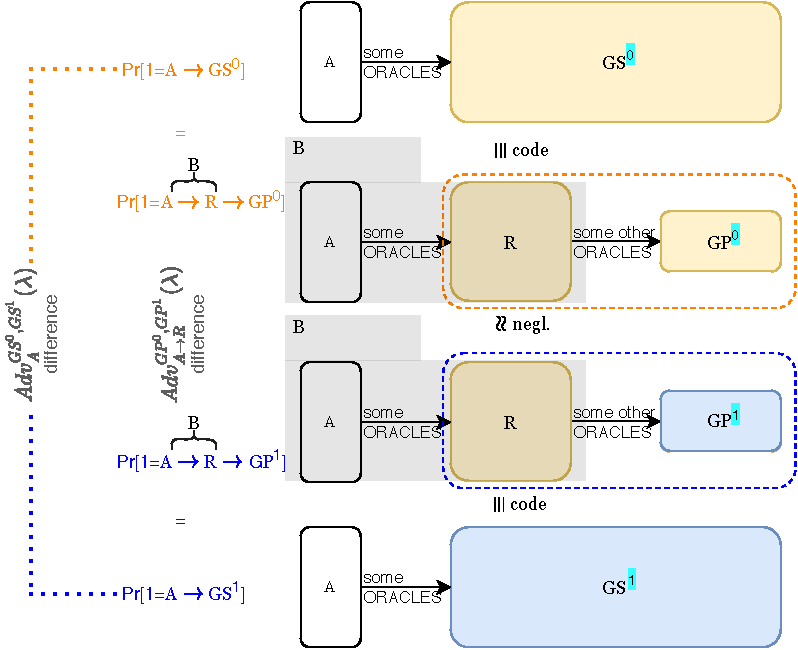
\includegraphics[width=0.6\textwidth]{figs/reduction}
\caption{\label{fig:reduction-example}New adversary $\bdv=\adv\circ\M{R}$}
\end{center}
\vspace{-0.5cm}
\end{wrapfigure}

In cryptography, we are often interested in proving the security of cryptographic systems or protocols. However, cryptography doesn't yet have methods of proving things secure from first principles (cf. the \textbf{P} vs. \textbf{NP} discussion in Section~\ref{ssec:assumptions}). Therefore, we are left with proving the security of systems \emph{assuming} that some (hopefully) well-understood and (typically) widely-used primitives are secure. Proofs of this type are done using reductions, which we explain in this section.

First, let's go over the general idea of a reduction proof.
Let's say that we want to prove the security of some system $S$, under the assumption that primitive $P$ is secure. In a reduction proof, we do this via a \emph{proof by contradiction}\footnote{Those familiar with formal logic will recognize this as modus ponens, i.e., $A\Rightarrow B$ is equivalent to $\neg B\Rightarrow \neg A$.} (which can take some time to get used to): we assume that $S$ is \emph{insecure} and prove that $P$ is then also insecure. If we can carry out such a proof, we can then argue that $S$ is secure. After all, if $S$ were insecure, then our proof would say that $P$ is also insecure, which is this in contradiction to our assumption that $P$ is \emph{secure}.

So, how do we prove that $S$ being insecure implies $P$ being insecure? Here it is important to realize what it means for $S$ to be insecure. It means that there is some (efficient) adversary $\adv$ that can break the security of $S$. Similarly, to prove that $P$ is insecure, we have to provide a new efficient adversary $\bdv$ that can break it. Due to our assumption of $\adv$ breaking $S$, we are allowed to use $\adv$ in the code of $\bdv$. As we don't know the \emph{code} of $\adv$, our construction of $\bdv$ needs to use $\adv$ in a black-box way. In particular, we can't make any assumptions about the precise functioning of $\adv$, except for knowing that $\adv$ breaks $S$.

Thus, we construct adversary $\bdv$ as a \emph{composition} of $\adv$ and a \emph{package} $\M{R}$, the latter of which we call reduction. A package is a generalization of the notion of a \emph{game} which we introduced in Section~\ref{ssec:security-games}. Namely, a package $\M{R}$ \emph{provides} oracles, denoted $[\rightarrow\M{R}]$, and also \emph{calls} oracles, denoted $[\rightarrow\M{R}]$. Now, in fact, an adversary can be seen as a package, too---it doesn't provide any oracles, it just calls some. So, e.g., to practice our language, we can say that $\adv$ and $\M{R}$ have \emph{matching} oracles and dependencies, namely $[\adv\rightarrow]=[\rightarrow\rdv]$, i.e., the oracles that $\adv$ calls are the oracles that $\M{R}$ provides. We use the $\rightarrow$ notation to write composition, namely, we define the adversary $\bdv$ as
\[\bdv:=\adv\rightarrow\M{R}.\]

We describe our reductions explicitly by giving the code of the oracles of the reduction. Namely, we consider the usual case that the security of $P$ is defined as the indistinguishability between a real game $\M{GP}^0$
and an ideal game $\M{GP}^1$. Let us further consider that the security of $S$ is defined as the indistinguishability between
a real game $\M{GS}^0$ and an ideal game $\M{GS}^1$. Then a reduction $\M{R}$ from the security of $S$ to the security of $P$
is an (efficient!) package $\M{R}$, written in pseudo-code. And we need that if $\adv$ is successful in distinguishing $\M{GP}^0$ and 
$\M{GP}^1$, then $\bdv:=\adv\rightarrow\M{R}$ is successful in distinguishing $\M{GS}^0$ from $\M{GS}^1$. The easiest case is,
if for all adversaries $\adv$, it holds that
\begin{equation}\label{lalaland1}
\mathsf{Adv}^{\M{GS}^0,\M{GS}^1}_\adv(\lambda)=\mathsf{Adv}^{\M{GP}^0,\M{GP}^1}_{\adv\rightarrow\M{R}}(\lambda).
\end{equation}
With Equation~\ref{lalaland} at hand, we can prove\footnote{See Lecture Notes 3 and Lecture Video 4, minutes 16:30 and 27:56, for a concrete such argument: The main reason that code equivalence implies that two games behave exactly the same and thus, and adversary has exactly the same probability against the two games. We use this argument a lot in this course.}  that for all adversaries $\adv$, it holds that 
and thus, if there is an efficient adversary $\adv$ which has non-negligible advantage against the pair $(\M{GS}^0,\M{GS}^1)$,
then there is also an efficient adversary $\adv\rightarrow\M{R}$ against the pair $(\M{GP}^0,\M{GP}^1)$ which has the same
advantage. However, we assume that there is no efficient $\bdv$ with non-negligible advantage $\mathsf{Adv}^{\M{GP}^0,\M{GP}^1}_{\bdv}$, thus taking $\bdv=\adv\rightarrow\M{R}$ leads to a contradiction. In conclusion, there cannot be an efficient $\adv$ such that $\mathsf{Adv}^{\M{GS}^0,\M{GS}^1}_\adv$ is non-negligible. The \emph{core argument}, here, is that (1) $\adv\rightarrow\M{R}$ is efficient (i.e., PPT) whenever $\adv$ is efficient, and (2) Equation~\ref{lalaland1}.

How can we prove that Equation~\ref{lalaland1} holds? We can show this by establishing that
\begin{align}
\notag          &\M{GS}^0\stackrel{\text{code}}{\equiv}\M{R}\rightarrow\M{GP}^0\text{ and }\\
\label{lalaland}&\M{GS}^1\stackrel{\text{code}}{\equiv}\M{R}\rightarrow\M{GP}^1,
\end{align}
that is, that $\M{GS}^0$ has the same input-output behaviour as $\M{R}\rightarrow\M{GP}^0$
and that $\M{GS}^1$ has the same input-output behaviour as $\M{R}\rightarrow\M{GP}^1$.
Because if this holds, then we can replace $\M{GS}^0$ by $\M{R}\rightarrow\M{GP}^0$
and $\M{GS}^1$ by $\M{R}\rightarrow\M{GP}^1$ and can prove Equation~\ref{lalaland1} as follows:
\begin{align*}
&\mathsf{Adv}^{\M{GS}^0,\M{GS}^1}_\adv(\lambda)\\
=&\abs{\prob{1=\adv\rightarrow\M{GS}^0}-\prob{1=\adv\rightarrow\M{GS}^1}}\\
=&\abs{\prob{1=\adv\rightarrow(\M{R}\rightarrow\M{GP}^0)}-\prob{1=\adv\rightarrow(\M{R}\rightarrow\M{GP}^1)}}\\
=&\abs{\prob{1=(\adv\rightarrow\M{R})\rightarrow\M{GP}^0}-\prob{1=(\adv\rightarrow\M{R})\rightarrow\M{GP}^1}}\\
=&\mathsf{Adv}^{\M{GP}^0,\M{GP}^1}_{\adv\rightarrow\M{R}}(\lambda)
\end{align*}
(Note that we usually don't write the brackets, we just include them here for emphasis.)

We now want to define the notion of a reduction formally. To do this, let us first include a formal definition of 
a \emph{package}.
\begin{definition}[Package]
A package $\M{R}$ consists of a set of oracles, denoted $[\rightarrow \M{R}]$,
which are defined by pseudo-code that operates on shared \emph{state variables} and makes calls to oracles in $[\M{R}\rightarrow]$,
which are called the \emph{dependencies} of $\M{R}$. Oracles in $[\rightarrow \M{R}]$
can only call oracles in $[\M{R}\rightarrow]$, they cannot call oracles in $[\rightarrow \M{R}]$.
(This is important for interpretation of code particularly if an oracle name $\O{O}$ is contained 
in $[\M{R}\rightarrow]$ and $[\rightarrow \M{R}]$.)
\end{definition}
\begin{definition}[Sequential Package Composition $\&$ Inlining]
If two packages $\M{R}$ and $\M{G}$ have \emph{matching interfaces}, i.e.,
$[\M{R}\rightarrow]\subseteq[\rightarrow\M{G}]$, then we can write
$\M{R}\rightarrow\M{G}$ for their composition which is defined by
inlining the code of the oracles of $\M{G}$ into the oracle of $\M{R}$,
i.e., if oracle $\O{O}\in[\rightarrow\M{G}]$ is defined as $\textit{code}(x);\pcreturn a$
and the pseudocode of oracle $\O{O}'\in[\rightarrow\M{R}]$ contains the line
$b\gets \O{x}$, then this line is replaced by $b\gets\textit{code}(x)$. Note that
when inlining, state variables might need to be renamed in order to avoid collisions.
\end{definition}

While Equation~\ref{lalaland1} was crucial in our argument, let us reflect on whether we need the actual Equation~\ref{lalaland1} or whether there are variants of it that would suffices. Actually, we only need an argument which justifies that if $\mathsf{Adv}^{\M{GS}^0,\M{GS}^1}_\adv$ is non-negligible, then $\mathsf{Adv}^{\M{GP}^0,\M{GP}^1}_{\adv\rightarrow\M{R}}$ is non-negligible. Any of the following inequalities would establish this desired result as well:
\begin{align*}
\mathsf{Adv}^{\M{GS}^0,\M{GS}^1}_\adv(\lambda)&\leq\mathsf{Adv}^{\M{GP}^0,\M{GP}^1}_{\adv\rightarrow\M{R}}(\lambda)\\
\mathsf{Adv}^{\M{GS}^0,\M{GS}^1}_\adv(\lambda)&\leq 2\cdot\mathsf{Adv}^{\M{GP}^0,\M{GP}^1}_{\adv\rightarrow\M{R}}(\lambda)\\
\mathsf{Adv}^{\M{GS}^0,\M{GS}^1}_\adv(\lambda)&\leq \O{poly}(\lambda)\cdot\mathsf{Adv}^{\M{GP}^0,\M{GP}^1}_{\adv\rightarrow\M{R}}(\lambda)\\
\mathsf{Adv}^{\M{GS}^0,\M{GS}^1}_\adv(\lambda)&\leq \O{poly}(\lambda)\cdot\sqrt{\mathsf{Adv}^{\M{GP}^0,\M{GP}^1}_{\adv\rightarrow\M{R}}(\lambda)}\\
\mathsf{Adv}^{\M{GS}^0,\M{GS}^1}_\adv(\lambda)&\leq \O{poly}(\lambda)\cdot\sqrt[5]{\mathsf{Adv}^{\M{GP}^0,\M{GP}^1}_{\adv\rightarrow\M{R}}(\lambda)}
\end{align*}
The reason that all of these inequalities work is that by multiplying (or dividing) by constants, polynomials and squaring (or taking square roots), a negligible function cannot become non-negligible (or vice versa). We are almost ready to state the notion of a reduction, but actually, we still need to make this statement a bit more general. The reason is that often, we have more than one algorithm $\M{R}$, and, e.g., might have inequalities such as 
\begin{equation}\label{lalaland12}
\mathsf{Adv}^{\M{GS}^0,\M{GS}^1}_\adv(\lambda)=\mathsf{Adv}^{\M{GP}^0,\M{GP}^1}_{\adv\rightarrow\M{R}_1}(\lambda)+\mathsf{Adv}^{\M{GP}^0,\M{GP}^1}_{\adv\rightarrow\M{R}_2}(\lambda),
\end{equation}
for two different, efficient $\M{R}_1$ to $\M{R}_1$. This equation still suffices, since the sum of two negligible functions is negligible again, and if $\mathsf{Adv}^{\M{GS}^0,\M{GS}^1}_\adv$ was non-negligible, then $\mathsf{Adv}^{\M{GP}^0,\M{GP}^1}_{\adv\rightarrow\M{R}_1}$ or 
$\mathsf{Adv}^{\M{GP}^0,\M{GP}^1}_{\adv\rightarrow\M{R}_2}$ would need to be non-negligible. As you can imagine, we can also combine this flexibility: Have \emph{several} efficient $\M{R}_i$ and some complex equation. To cross-refer to the lectures, let me mention here an inequality which we use in Lecture Notes 4:
\begin{align}
   \notag&\mathsf{Adv}^{\M{Gunf\text{-}cma}_{\m_f}^0,\M{Gunf\text{-}cma}_{\m_f}^1}_{\m_f,\adv}(\lambda)\\
   \notag\leq&\mathsf{Adv}^{\M{Gprf}^0,\M{Gprf}^1}_{f,\adv\rightarrow\M{R}_1}(\lambda)\\
	       &\label{lalaland123}+\mathsf{Adv}^{\M{Gprf}^0,\M{Gprf}^1}_{f,\adv\rightarrow\M{R}_2}(\lambda)+\frac{\O{poly}_{\adv}(\lambda)}{2^\lambda},
\end{align}
Here, we add two advantages and some negligible term $\frac{\O{poly}_{\adv}(\lambda)}{2^\lambda}$, where $\O{poly}_{\adv}$ is
some polynomial which depends on the adversary (in this case an upper bound on the number of queries that $\adv$ makes).
Thus, also Inequality~\ref{lalaland123} suffices to establish that if there is no efficient adversary such that 
\[\mathsf{Adv}^{\M{Gprf}_f^0,\M{Gprf}_f^1}_{f,\bdv}\] is non-negligible, then there is also no efficient adversary such
that \[\mathsf{Adv}^{\M{Gunf\text{-}cma}_{\m_f}^0,\M{Gunf\text{-}cma}_{\m_f}^1}_{\m_f,\adv}\] is non-negligible.

\begin{quote}
How do we know which combination is the right one in which situation?
\end{quote}

We don't really know this. Moreover, there are
often more than one right way to do this. In essence, any approach that works is good, and we will see many such
examples of proofs in this book,
 so they will hopefully become familiar over time.

Let us now state the notion of a reduction:
\begin{definition}[Reduction]
We call a package $\M{R}$ a reduction from the indistinguishability of $\M{GS}^0$ and  $\M{GS}^1$ to the indistinguishability of 
$\M{PS}^0$ and  $\M{PS}^1$, if
\begin{itemize}
\item $\M{R}$ is efficient, i.e., probabilistic polynomial-time (PPT), and
\item for any efficient adversary $\adv$, it holds that if $\mathsf{Adv}^{\M{GS}^0,\M{GS}^1}_\adv$ is non-negligible, then
      $\mathsf{Adv}^{\M{GP}^0,\M{GP}^1}_{\adv\rightarrow\M{R}}$ is non-negligible.
\end{itemize}
Additionally, we call two packages $\M{R}_1$ and $\M{R}_2$ reductions from the indistinguishability of $\M{GS}^0$ and  $\M{GS}^1$ to the indistinguishability of 
$\M{PS}^0$ and  $\M{PS}^1$, if
\begin{itemize}
\item $\M{R}_1$ and $\M{R}_2$ are efficient, i.e., probabilistic polynomial-time (PPT), and
\item for any efficient adversary $\adv$, it holds that if $\mathsf{Adv}^{\M{GS}^0,\M{GS}^1}_\adv$ is non-negligible, then
      $\mathsf{Adv}^{\M{GP}^0,\M{GP}^1}_{\adv\rightarrow\M{R}_1}$ or $\mathsf{Adv}^{\M{GP}^0,\M{GP}^1}_{\adv\rightarrow\M{R}_2}$ is non-negligible.
\end{itemize}
In this case, we refer to $\M{R}_1$ and $\M{R}_2$ as a reductions, even though one of them alone does not match the first
part of the definition.
\end{definition}
Potentially, we could have also more than two reductions $\M{R}_i$, but we are not aware of any such example,
so we do not generalize the definition.


\iffalse
So, how do we prove that $S$ being insecure implies $P$ being insecure? Here it is important to realize what it means for $S$ to be insecure. It means that there is some adversary $\adv$ that can break the security of $S$. Similarly, to prove that $P$ is insecure, we have to provide an adversary $R$ that can break it. However, due to our assumption, we are allowed to use $\adv$ in the code of $R$. Note that we don't know the \emph{code} of $\adv$, so $R$ can only use $\adv$ in a black-box way, and we can't make any assumptions about the precise functioning of $\adv$.

Reduction proofs can be carried out explicitly, by defining $R$ in pseudocode. However, a major benefit of the framework we're using is to simplify proofs of this type. Often, we can do a reduction proof just using package composition diagrams for the two systems in question. This is because the reductions we want to construct are often simply some part of the package composition we are working with. The next section does reduction proofs in detail, so reading those might be the best way of getting to grips with this idea. Here, we will only discuss the idea in general, algebraic terms. Figure~\ref{fig:reduction-example} presents the situation graphically, so you might like to look at it while reading the following.

\begin{wrapfigure}{R}{0.6\textwidth}
\vspace{-0.5cm}
\begin{center}
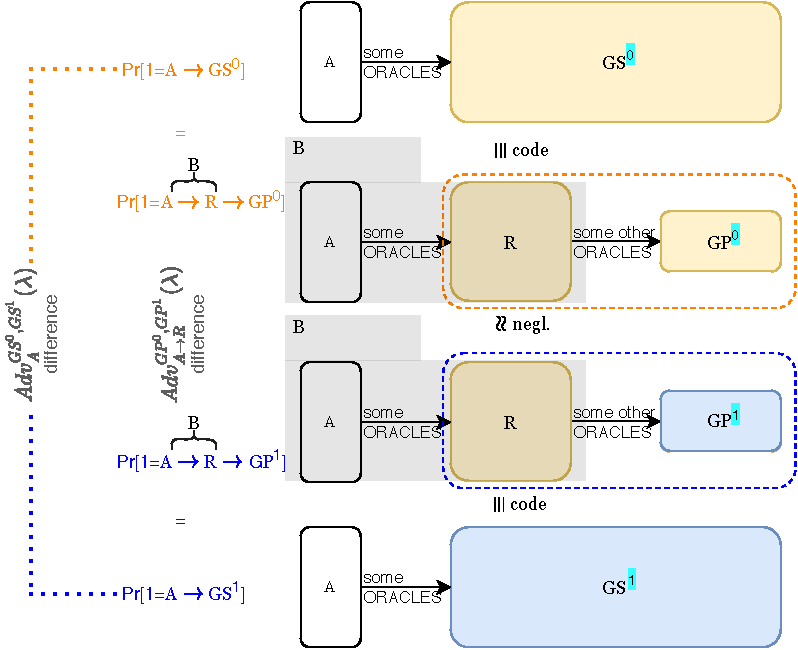
\includegraphics[width=0.6\textwidth]{figs/reduction}
\caption{\label{fig:reduction-example}Reduction $\rdv=\adv\circ\M{N}$}
\end{center}
\vspace{-0.5cm}
\end{wrapfigure}

Let us say we are trying to prove that some system $S$ is secure assuming that primitive $P$ is secure. Let us further posit that security of  $S$ is defined by indistinguishability of the real and ideal games $\M{S}^0$ and $\M{S}^1$, depicted in orange and blue, respectively. Similarly, consider that the security of $P$ is defined by the indistinguishability of the real game $\M{P}^0$ and the ideal game $\M{P}^1$. Now, we set out to prove that $P$ is insecure assuming that $S$ is. The assumption gives us an adversary that can break the security of $S$. This means, specifically, that the composition $\adv\circ\M{S}^0$ returns $1$ with much higher (or much lower) probability than the composition
$\adv\circ\M{S}^1$ so that the difference between these two probabilities is some high enough value $\epsilon$. Now, let us say that we can re-write $\M{S}^0$ as $\M{N}\circ\M{P}^0$ for some package $\M{N}$ and let us consider the situation that $\M{S}^1=\M{N}\circ\M{P}^1$ for the same package $\M{N}$. Now, we can rewrite the $\M{S}^0$ and $\M{S}^1$ into $\M{N}\circ\M{P}^0$ and $\M{N}\circ\M{P}^1$ (illustrated by orange and blue dashed lines, respectively). As the systems still behave the same, the probabilities remain unchanged and $\epsilon$ is now also the difference between $\adv \circ \M{N} \circ \M{P}^0$ returning $1$ and $\adv \circ \M{N} \circ \M{P}^1$ returning $1$.

Now, we can construct our reduction $R$: it is simply $\adv \circ \M{N}$. If the composition $\adv \circ (\M{N} \circ \M{P}^b)$ returns $1$, so must the composition $(\adv \circ \M{N}) \circ \M{P}^b = R \circ \M{P}^b$. Thus, in conclusion, we can argue that the security of $S$ (i.e., an adversary's distinguishing advantage between $\M{S}^0$ and $\M{S}^1$) is equal to the security of $P$ (i.e., the distinguishing advantage of a different adversary between $\M{P}^0$ and $\M{P}^1$). 

This is the general form that reduction proofs in this course follow. The problem often is not so simple, i.e., sometimes, we need to consider two slightly different packages $\M{N}$ and $\M{N'}$ which actually behave in the same way (or almost the same way) but have slightly different code. In this case, the same type of argument still goes through as long as we can show that $\M{N}$ and $\M{N'}$ are \emph{code-equivalent}. 
\fi

We already mentioned the technique of proving \emph{code-equivalence} several time. We turn to code-equivalence in the next section.
\subsection{Code equivalence}
A recurring task we will encounter is proving that two pieces of code behave in the same way. These pieces of code could be algorithms, packages or compositions of packages. For example, in proving relationships between primitives, we often wish to prove that some piece of code behaves in the same way as a primitive. One of the main benefits of using pseudocode as our model of computation is being able to do proofs of this type rigorously. In this section, we will discuss what we mean by two pieces of code behaving in the same way, and the ways to prove that they do.

The way we model two pieces of code behaving in the same way is by the concept of \emph{code equivalence}. Two pieces of code being code-equivalent means that, after applying certain transformations to the code of one or both of them, they have exactly the same code. These transformations should be ones that don't alter the input-output behaviour of the code. Then, we can say that two pieces of code-equivalent code have the same input-output behaviour. Here is a list of common transformations
\begin{itemize}
    \item Inlining the code of oracles
    \item Renaming variables (in an injective way so that distinct variables are renamend to two distinct variables as well)
    \item Assigning an additional variable if that variable is not read
    \item Removing a variable assignment if that variable is not read
    \item Move a line of code if the variables which appear in it do not appear in the code-lines in between the original and the final location of the code line
\end{itemize}
This list is not exhaustive: there are other transformations you can use as well. However, if you use other transformations, you should justify why they have no effect on the input-output behaviour of the code.

The described transformations are very formal: it can be checked mechanically that they don't affect the input-output behvaiour. Using only such transformations makes proofs very precise. However, this level of precision brings practical problems with it: some types of argument are challenging to couch just in terms of code. Therefore, proofs in this course are allowed to use higher-level reasoning as well. However, when you deviate from purely code-based arguments, you should be very careful: this is where mistakes can easily happen.

Before we move on to describing and justifying these transformations, we should say a few words about running time. You might have noticed that some of the transformations above change the running time of the code by removing or adding lines\footnote{For those familiar with complexity theory: the transformations described only change runtime by constant amounts, but there might be more complex situations where code equivalent pieces of code are in different complexity classes.}. Of course, if we want to argue about running time, then these changes in running time need to be taken into consideration. However, when we only want to argue about \emph{code-equivalence}, then we only need to make claims about the \emph{input-output behaviour}.

The rest of this section is devoted to discussing the details of how to write proofs using such transformations. We use the algebraic notation which we introduced in Section~\ref{ssec:pseudocode-defs}.

\paragraph{Inlining}
When writing a code-equivalence proof, our first obstacle is often that the systems are defined in terms of package composition, and we cannot directly compare the code. To be able to compare the two systems, we first turn them into a single package with self-contained oracles. We do this by \emph{inlining}.
Consider the simple package composition
\[\M{M}\circ\M{N}\;\;\;\text{ or }\;\;\;\stackrel{\O{O}_1}{\longrightarrow}\M{M}\stackrel{\O{O}_2}{\longrightarrow}\M{N},\text{
        using graph-notation for the latter.}\]
There is some line of the form $y\gets\O{O}_2(x)$ in the code of $\O{O}_1$ since it calls the oracle $\O{O}_2$.
Let us describe the code of oracle $\O{O}_2(x)$ in package $\M{N}$ generally as ``$\V{code}(x);\ \pcreturn z$''. Then, we can inline $\M{N}$ into $\M{M}$ by replacing, in the code of $\O{O}_1$, the line ``$y\gets\O{O}_2(x)$'' by ``$\V{code}(x);\ y\gets z$''. Inlining is useful to prove \emph{code equivalence} between a package composition $\M{M}\circ\M{N}$ and some other package $\M{P}$. We write this as
\[\M{M}\circ\M{N}\stackrel{\text{code}}{\equiv}\M{P}\]

We need to be careful when inlining, because some of the variable names might collide. Programming language theory has good methods to deal with situations like this, for example by first renaming each variable before inlining such that collisions in inlining are avoided, e.g., by
prepending each variable name by the name of the package. Since we are not doing formal computer science, we will simply be careful to avoid such clashes in variable names by using globally unique variable names in a package composition\footnote{This being said, if you notice any such clashes, let Chris or Valtteri know.} or by doing renaming in an ad-hoc fashion.

Another case that requires careful treatment is the \emph{parallel} compositions of packages. Essentially, one package can only ever be inlined into a \emph{single} other package. That is, if two packages $\M{L}$ and $\M{M}$ both make calls to a package $\M{N}$, then we first need to turn the $\M{L}$ and $\M{M}$ into a single package, denoted $\tfrac{\M{L}}{\M{M}}$ (see Section \ref{ssec:pseudocode-defs} for details on notation). In practice we simply write a package that contains all the oracles of packages $\M{L}$ and $\M{M}$. More formally, we have to define a package whose state contains the union of the state of $\M{L}$ and $\M{M}$ and which provides the oracles $\outinterface{\tfrac{\M{L}}{\M{M}}}:=\outinterface{\M{L}}\cup\outinterface{\M{M}}$. Note that this package is only well-defined if $\outinterface{\M{L}}\cap\outinterface{\M{M}}=\emptyset$. After joining $\M{L}$ and $\M{M}$ into $\tfrac{\M{L}}{\M{M}}$, we can now inline $\M{N}$ into $\tfrac{\M{L}}{\M{M}}$.

Recall the we discussed inlining as a tool for code equivalence proofs between package compositions. Now, inlining along only suffices to prove code equivalence between two packages, if their code is indeed identical. But often, it is not exactly identical, but rather differs in small ways that do not affect the behavior of the program.

\paragraph{Code Rewriting}
There rest of the transformations described in the beginning of this subsection are examples of \emph{code rewriting}. These are ways to change the code without altering its behaviour. First off, we have \emph{variable renaming}. This means replacing all occurrences of a variable-name $x$ in the code with a new variable-name. Since variable names are arbitrary, it doesn't affect behaviour to change them. There is one caveat: the new variable name has to be \emph{fresh}. This means that it doesn't occur anywhere in the code before the renaming.

Next, there are two related transformations that add and remove code. We can \emph{assign an additional variable}, as long as the additional variable has a fresh name, this variable is never read and thus adding this code line does not behave the behavior of the system. The inverse of assigning an additional variable is \emph{removing a line of code}. We can do this, provided that the line assigns a variable that is not read anywhere else in the code: it then cannot affect the behaviour of the system.

The final transformation is \emph{moving a line of code} to an earlier or later position in the code. We can do this if the computations in between are \emph{independent} of the line being moved, meaning that they do not share any variables.

As we already mentioned, you can also use other transformations, provided you argue for why they do not affect outside behavior of the code.

\subsection{Recipes and principles}
It has been asked: How to we come up with reductions? How do we knwo whether we need one or two reductions? Our own recipe for this is as follows. Say, we want to reduce the indistinguishability of two big games $\M{Gbig}^0$ and $\M{Gbig}^1$ to the indistinghuishability of two small games $\M{Gsmall}^0$ and $\M{Gsmall}^1$. The first thing we try is to come up with a reduction $\mathcal{R}$ such that the following two hold:

\begin{align}
    \label{eqn:smallbig0} & \mathcal{R}\rightarrow\M{Gsmall}^0\stackrel{\text{code}}{\equiv}\M{Gbig}^0 \\
    \label{eqn:smallbig1} & \mathcal{R}\rightarrow\M{Gsmall}^1\stackrel{\text{code}}{\equiv}\M{Gbig}^1
\end{align}

If we can manage to find such an $\rdv$, then this is great, because from (\ref{eqn:smallbig0}) and (eqn:smallbig1), we can directly derive that the advantage of an adversary $\mathcal{A}$ in distinguishing between $\M{Gsmall}^0$ and $\M{Gsmall}^1$ is upper bounded by the advantage of the (composed) adversary $\mathcal{A}\rightarrow\mathcal{R}$ in distinguishing between $\M{Gbig}^0$ and $\M{Gbig}^1$. If we can find a reduction $\rdv$ such that (\ref{eqn:smallbig0}) and (eqn:smallbig1) holds, then we typically find it by looking at the construction whose security we model and our reduction mimics the behaviour of the construction---we call this a reduction-analogous-construction (CAR).

However, if we can't find a reduction such that  (\ref{eqn:smallbig0}) and (eqn:smallbig1) holds, then we need more than one reduction. In this case, we typically come up with two reductions $\mathcal{R}_0$ and $\mathcal{R}_1$ such that:

\begin{align}
    \label{eqn:smallbig00} & \mathcal{R}_0\rightarrow\M{Gsmall}^0\stackrel{\text{code}}{\equiv}\M{Gbig}^0 \\
    \label{eqn:smallbig11} & \mathcal{R}_1\rightarrow\M{Gsmall}^0\stackrel{\text{code}}{\equiv}\M{Gbig}^1
\end{align}

Now, we are not done yet, we still need to compare $\mathcal{R}_0\rightarrow\M{Gsmall}^1$ and $\mathcal{R}_1\rightarrow\M{Gsmall}^1$ (observe that now the bit is $$1$$ in the games) and somehow argue/prove/explain that every adversary can distinguish them only with negligible probability.
\subsection*{What's next}
The next Section describes constructions and states theorems for the constructions. The proofs for these statements are given
in Section~\ref{section:proofs}. The techiques described in this section will be used in most of those proofs.

\clearpage
\section{Proofs} \label{section:proofs}
This Section goes over concrete security proofs, using all the tools of the previous sections. The proofs serve two purposes. First, they give concrete examples of doing the types of security proofs this book has been focused on. Second, they give proofs of interesting results in a uniform format that is easy to refer to.

There are no dependencies between the proofs given here, so you can go to whichever subsection interests you. When reading a proof, you might have to refer to Section \ref{section:definitions} for any unfamiliar notation and to the definitions of the relevant primitives in Section \ref{section:primitives}.
\subsection{Proofs for One-Way Function Transformations}
The proofs in this section do not fully follow the pattern outlined in the previous section. The reason is that the proofs in this section make statements about one-way functions, which are best formulated as win-loose security experiments, so we just use the pattern of arguing by contradiction, but not the more rigid structure presented in the previous section. This being said, the statements we prove in these sections are not very deep (even though some technicalities occur), and the proofs might be a good warm-up for later proofs, especially since they nicely showcase how to transform an adversary against some ``fancy'' OWF into an adversary against the underlying basic OWF.

\begin{figure}
\begin{codebox}
	\begin{center}
		\begin{pchstack}
  		\begin{pcvstack}
				  \procedure{$\adv^f_{\text{app-zer}}(1^\lambda,y)$}{
					y'\gets y||0^{\abs{x}}\\
					x'\sample \adv_g(1^\lambda,y')\\
					\pcreturn x'}			
					\pcvspace
				  \procedure{$\adv^f_{\text{app-ones}}(1^\lambda,y)$}{
					y'\gets y||0^{\abs{x}}\\
					x'\sample \adv_g(1^\lambda,y')\\
					\pcreturn x'}
  		\end{pcvstack}
					\pchspace
				  \procedure{$\adv^f_{\text{leak-l}}(1^\lambda,y)$}{
					b\sample\bin\\
          m\gets \lambda-b\\
					x_\ell\sample\bin^m\\
					y'\gets x_\ell||y\\
					\lambda'\gets \lambda+m\\
					x'\sample \adv_g(1^{\lambda'},y')\\
					x^{\prime\prime}\gets x'_{m+1..\abs{x'}}\\
					\pcreturn x^{\prime\prime}
					}
					\pchspace
				  \procedure{$\adv^f_{\text{leak-r}}(1^\lambda,y)$}{
					b\sample\bin\\
          m\gets \lambda\\
					x_r\sample\bin^{\lambda+b}\\
					y'\gets y||x_r\\
  				\lambda'\gets \lambda+b+m\\
					x'\sample \adv_g(1^{\lambda'},y')\\
					x^{\prime\prime}\gets x'_{1..m}\\
					\pcreturn x^{\prime\prime}
					}
					\pchspace
				  \procedure{$\adv^f_{\text{ign-l}}(1^\lambda,y)$}{
					m\gets \left\lfloor{\tfrac{\abs{x}}{2}}\right\rfloor\\
					\\
					x_r\gets x_{m+1..\abs{x}}\\					
					y\gets f(x_r)\\
					\pcreturn y}
					\pchspace
				  \procedure{$\adv^f_{\text{ign-r}}(1^\lambda,y)$}{
					m\gets \left\lfloor{\tfrac{\abs{x}}{2}}\right\rfloor\\
					x_\ell\gets x_{1..m}\\
					\\					
					y\gets f(x_\ell)\\
					\pcreturn y}
		\end{pchstack}
	\end{center}
	\end{codebox}
	\caption{Constructions of adversaries against the underlying OWF $f$ assuming an adversary against the construction $g$.\label{fig:owfreductions}}
	\end{figure}

\paragraph{Proof of Theorem~\ref{thm:owf-app-zer}}
Recall that Theorem~\ref{thm:owf-app-zer} states that if $f$ is a one-way function, then $g^f_{\text{app-zer}}$ and $g^f_{\text{app-ones}}$ are one-way functions, too. We first prove the statement for $g^f_{\text{app-zer}}$.
In order to prove that $g^f_{\text{app-zer}}$ \emph{is} a one-way function, we will first assume towards contradiction that it \emph{isn't}. We will see that this leads us to a contradiction with the assumption that $f$ is a one-way function. Thus, if $f$ is a one-way function, then
$g^f_{\text{app-zer}}$ must be a one-way function, too. We now go into the details of this proof.

Assume towards contradiction that $g^f_{\text{app-zer}}$ is not a one-way function. Then, by definition of one-wayness (Security Definition~\ref{secdef:owf}), there must be a PPT adversary $\adv_g$ against $g^f_{\text{app-zer}}$ such that $\prob{1={\mathsf{Exp}}_{g^f_{\text{app-zer}},\adv_g}^{\mathsf{OW}}(1^\lambda)}$ is non-negligible. From $\adv_g$, we will now construct another PPT adversary $\adv^f_{\text{app-zer}}$ such that 
\begin{equation}\label{eq:reductionowfzeroes}
\prob{1={\mathsf{Exp}}_{f,\adv^f_{\text{app-zer}}}^{\mathsf{OW}}(1^\lambda)}=\prob{1={\mathsf{Exp}}_{g^f_{\text{app-zer}},\adv_g}^{\mathsf{OW}}(1^\lambda)}
\end{equation}
and thus, $\prob{1={\mathsf{Exp}}_{f,\adv^f_{\text{app-zer}}}^{\mathsf{OW}}(1^\lambda)}$ is non-negligible, too, leading to a contradiction with the one-wayness of $f$. Thus, all we are left to do is to prove the following claim.
\begin{claim}\label{claim:owfsimple}
For each PPT adversary $\adv_g$ against the one-wayness of $g^f_{\text{app-zer}}$, there exists a PPT adversary $\adv^f_{\text{app-zer}}$ against the one-wayness of $f$ such that Equation~\ref{eq:reductionowfzeroes} holds.
\end{claim}
To prove Claim~\ref{claim:owfsimple}, we need to construct $\adv^f_{\text{app-zer}}$, see the leftmost column of Figure~\ref{fig:owfreductions}. As $\adv^f_{\text{app-zer}}$ merely adds $\lambda$ many zeroes and else essentially has the same runtime as $\adv_g$, the adversary $\adv^f_{\text{app-zer}}$ is polynomial-time, since $\adv_g$ runs in polynomial-time and since the additional operations are only linear-time in $\lambda$. We now need to prove that Equation~\ref{eq:reductionowfzeroes} holds. We prove this by showing that, essentially, the two experiments behave in the same way. I.e., below, we start with experiment ${\mathsf{Exp}}_{f,\adv^f_{\text{app-zer}}}^{\mathsf{OW}}(1^\lambda)$, where from the left-most column to the second column, we inline the code of ${\mathsf{Exp}}_{f,\adv^f_{\text{app-zer}}}^{\mathsf{OW}}(1^\lambda)$ (marked in grey). We also replace $y$ by $f(x)$ (marked in grey), since it is the same value.
\begin{center}
\begin{pchstack}
	  \procedure{${\mathsf{Exp}}_{f,\adv^f_{\text{app-zer}}}^{\mathsf{OW}}(1^\lambda)$}{
		x\sample\bin^\lambda\\
		y\gets f(x)\\
		x'\sample\adv^f_{\text{app-zer}}(1^\lambda,y)\\
		\\
		\pcassert \abs{x'}=\lambda\\
		\pcif f(x')=y:\\
		\pcind \pcreturn 1\\
		\pcreturn 0}
		    \pchspace
	  \procedure{${\mathsf{Exp}}_{f,\adv^f_{\text{app-zer}}}^{\mathsf{OW}}(1^\lambda)$}{
		x\sample\bin^\lambda\\
		y\gets f(x)\\
		\gamechange{$y'\gets y||0^\lambda$}\\		
		\gamechange{$x'\sample\adv_g(1^\lambda,y')$}\\
		\pcassert \abs{x'}=\lambda\\
		\pcif f(x')=\gamechange{$f(x)$}:\\
		\pcind \pcreturn 1\\
		\pcreturn 0}
		\pchspace
			  \procedure{${\mathsf{Exp}}_{g^f_{\text{app-zer}},\adv_g}^{\mathsf{OW}}(1^\lambda)$}{
		x\sample\bin^\lambda\\
		\gamechange{$y\gets f(x)||0^{\abs{x}}$}\\
		\\
		x'\sample\adv_g(1^\lambda,y)\\
		\pcassert \abs{x'}=\lambda\\
		\pcif \gamechange{$f(x')||0^{\abs{x'}}=f(x)||0^{\abs{x}}$}:\\
		\pcind \pcreturn 1\\
		\pcreturn 0}
				\pchspace
			  \procedure{${\mathsf{Exp}}_{g^f_{\text{app-zer}},\adv_g}^{\mathsf{OW}}(1^\lambda)$}{
		x\sample\bin^\lambda\\
		y\gets g^f_{\text{app-zer}}(x)\\
		\\
		x'\sample\adv_g(1^\lambda,y)\\
		\pcassert \abs{x'}=\lambda\\
		\pcif g^f_{\text{app-zer}}(x')=y:\\
		\pcind \pcreturn 1\\
		\pcreturn 0}
\end{pchstack}
\end{center}
The right-most experiment (column 4) contains the description of ${\mathsf{Exp}}_{g^f_{\text{app-zer}},\adv_g}^{\mathsf{OW}}(1^\lambda)$.
From column 4 to column 3, we inlined the code of $g^f_{\text{app-zer}}(x)$ twice and we replaced $y$ by its value. Now, the proof concludes by observing that column 2 and column 3 essentially contain the same code. We only need to observe the following: Checking $f(x')=f(x)$ (column 2) is the same as performing the same checks with $\lambda$ zeroes appended to it---note that at this point, both, $\abs{x}$ and  $\abs{x'}$ are equal to $\lambda$. In column 3, if we additionally rename variable $y$ to $y'$, we yield the same code.

\paragraph{Proof for $g^f_{\text{app-ones}}$} The proof for $g^f_{\text{app-ones}}$ is analogous to the proof for $g^f_{\text{app-zer}}$. We first assume towards contradiction that $g^f_{\text{app-ones}}$ is not a one-way function. This implies that there exists a PPT $\adv_g$ against $g^f_{\text{app-ones}}$ such that $\prob{1={\mathsf{Exp}}_{g^f_{\text{app-ones}},\adv_g}^{\mathsf{OW}}(1^\lambda)}$ is non-negligible.
We now need to prove the analogous claim to Claim~\ref{claim:owfsimple}, namely:
\begin{claim}\label{claim:owfsimple1}
For each PPT adversary $\adv_g$ against the one-wayness of $g^f_{\text{app-ones}}$, there exists a PPT adversary $\adv^f_{\text{app-ones}}$ against the one-wayness of $f$ such that the following equation holds.
\begin{equation}\label{eq:reductionowfones}
\prob{1={\mathsf{Exp}}_{f,\adv^f_{\text{app-ones}}}^{\mathsf{OW}}(1^\lambda)}=\prob{1={\mathsf{Exp}}_{g^f_{\text{app-ones}},\adv_g}^{\mathsf{OW}}(1^\lambda)}
\end{equation}
\end{claim}
Once we prove Claim~\ref{claim:owfsimple1}, we can conclude the existence of a PPT adversary against $f$ with non-negligible inverting probability and thus reach a contradiction. The proof of Claim~\ref{claim:owfsimple1} is analogous to the proof of Claim~\ref{claim:owfsimple}, just replace zeroes by ones at all positions. Let us include it here for completeness:
\begin{center}
\begin{pchstack}
	  \procedure{${\mathsf{Exp}}_{f,\adv^f_{\text{app-ones}}}^{\mathsf{OW}}(1^\lambda)$}{
		x\sample\bin^\lambda\\
		y\gets f(x)\\
		x'\sample\adv^f_{\text{app-ones}}(1^\lambda,y)\\
		\\
		\pcassert \abs{x'}=\lambda\\
		\pcif f(x')=y:\\
		\pcind \pcreturn 1\\
		\pcreturn 0}
		    \pchspace
	  \procedure{${\mathsf{Exp}}_{f,\adv^f_{\text{app-ones}}}^{\mathsf{OW}}(1^\lambda)$}{
		x\sample\bin^\lambda\\
		y\gets f(x)\\
		\gamechange{$y'\gets y||1^\lambda$}\\		
		\gamechange{$x'\sample\adv_g(1^\lambda,y')$}\\
		\pcassert \abs{x'}=\lambda\\
		\pcif f(x')=\gamechange{$f(x)$}:\\
		\pcind \pcreturn 1\\
		\pcreturn 0}
		\pchspace
			  \procedure{${\mathsf{Exp}}_{g^f_{\text{app-ones}},\adv_g}^{\mathsf{OW}}(1^\lambda)$}{
		x\sample\bin^\lambda\\
		\gamechange{$y\gets f(x)||1^{\abs{x}}$}\\
		\\
		x'\sample\adv_g(1^\lambda,y)\\
		\pcassert \abs{x'}=\lambda\\
		\pcif \gamechange{$f(x')||1^{\abs{x'}}=f(x)||1^{\abs{x}}$}:\\
		\pcind \pcreturn 1\\
		\pcreturn 0}
				\pchspace
			  \procedure{${\mathsf{Exp}}_{g^f_{\text{app-ones}},\adv_g}^{\mathsf{OW}}(1^\lambda)$}{
		x\sample\bin^\lambda\\
		y\gets g^f_{\text{app-ones}}(x)\\
		\\
		x'\sample\adv_g(1^\lambda,y)\\
		\pcassert \abs{x'}=\lambda\\
		\pcif g^f_{\text{app-ones}}(x')=y:\\
		\pcind \pcreturn 1\\
		\pcreturn 0}
\end{pchstack}
\end{center}

The right-most experiment (column 4) describes ${\mathsf{Exp}}_{g^f_{\text{app-zer}},\adv_g}^{\mathsf{OW}}(1^\lambda)$.
From column 4 to column 3, we inlined the code of $g^f_{\text{app-zer}}(x)$ twice and we replaced $y$ by its value. Now, the proof concludes by observing that column 2 and column 3 essentially contain the same code. We only need to observe the following: Checking $f(x')=f(x)$ (column 2) is the same as performing the same checks with $\lambda$ zeroes appended to it---note that at this point, both, $\abs{x}$ and  $\abs{x'}$ are equal to $\lambda$. In column 3, if we additionally rename variable $y$ to $y'$, we yield the same code.


\clearpage
\subsection{Acknowledgements}
We are greatful to Eric Cornelissen, Eljon Harlicaj and Pihla Karanko for suggestions and careful proof-reading of the the book in its various forms. We thank Jan Winkelmann for inspiring discussions especially on notation and, in particular, for suggesting to list state and parameters explicitly in the package definitions. We thank Konrad Kohbrok and Markulf Kohlweiss for useful discussions and suggestions regarding the code-structuring and further formalizations. We thank Estuardo Alpirez Bock and Miika Leinonen for suggestions on the didactics and order of presentation. Last, but not least, thanks to all course participants who contributed to the improvement of the document by enriching our understanding of learning.

(Some of the acknowledgements are missing. If you feel you have contributed to the book, we would be very happy to add your name here.)
\printbibliography

\clearpage
\appendix
\section{Equivalent Notions of Advantage}\label{app:calculus}
In this appendix, we prove the following claim:
\begin{claim}
    It holds that
    \begin{equation*}
        2\cdot\tilde{\mathbf{Adv}}_\adv^{\M{G}^0,\M{G}^1}(\lambda)=\mathbf{Adv}_\adv^{\M{G}^0,\M{G}^1}(\lambda),
    \end{equation*}
    where
    \[\mathbf{Adv}_\adv^{\M{G}^0,\M{G}^1}(\lambda):=\abs{\prob{1 = \adv \circ \M{G}^0} - \prob{1 = \adv \circ \M{G}^1}}\]
    and
    \[\tilde{\mathbf{Adv}}_\adv^{\M{G}^0,\M{G}^1}(\lambda):=\abs{\probsub{b\sample\bin}{b = \adv \circ \M{G}^b} - \frac{1}{2}}.\]
\end{claim}
\begin{proof}
    \begin{align*}
        \mathbf{Adv}_\adv^{\M{G}^0,\M{G}^1}(\lambda)                                                                                      \\
        = & \abs{\prob{1 = \adv \circ \M{G}^0} - \prob{1 = \adv \circ \M{G}^1}}                                                           \\
        = & \abs{\prob{1 = \adv \circ \M{G}^1}-\prob{1 = \adv \circ \M{G}^0}}                                                             \\
        = & \abs{-\prob{1 = \adv \circ \M{G}^0} + \prob{1 = \adv \circ \M{G}^1}}                                                          \\
        = & \abs{(1-\prob{1 = \adv \circ \M{G}^0}) + \prob{1 = \adv \circ \M{G}^1} - 1}                                                   \\
        = & 2\cdot\abs{\frac{1}{2}\cdot (1-\prob{1 = \adv \circ \M{G}^0}) + \frac{1}{2}\cdot \prob{1 = \adv \circ \M{G}^1} - \frac{1}{2}} \\
        = & 2\cdot\abs{\frac{1}{2}\cdot \prob{0 = \adv \circ \M{G}^0} + \frac{1}{2}\cdot \prob{1 = \adv \circ \M{G}^1} - \frac{1}{2}}     \\
        = & 2\cdot\abs{\probsub{b\sample\bin}{b = \adv \circ \M{G}^b} - \frac{1}{2}}                                                      \\
        = & 2\cdot\tilde{\mathbf{Adv}}_\adv^{\M{G}^0,\M{G}^1}(\lambda)                                                                    \\
    \end{align*}
\end{proof}

\end{document}
